\documentclass[12pt,a4paper]{report}

\usepackage[a4paper,left=1.25in,right=1in,top=1in,bottom=1in]{geometry}
\usepackage[utf8]{inputenc}
\usepackage[T1]{fontenc}
\usepackage{mathptmx} % Times New Roman typography throughout
\usepackage{setspace}
\usepackage{titlesec}
\usepackage{tocloft}
\usepackage{graphicx}
\usepackage{booktabs}
\usepackage{longtable}
\usepackage{array}
\usepackage{tabularx}
\usepackage{amsmath,amssymb}
\usepackage{listings}
\usepackage{xcolor}
\usepackage{fancyhdr}
\usepackage{caption}
\usepackage{enumitem}
\usepackage{float}
\usepackage{tikz}
\usetikzlibrary{arrows.meta,positioning,shapes.geometric,fit,calc}
\usepackage[hidelinks]{hyperref}
\usepackage{url}

% 1.5 line spacing as per sample report
\onehalfspacing
\setlength{\parindent}{0.4in}
\setlength{\parskip}{4pt}

% Running headers and footers matching sample PDF exactly
\pagestyle{fancy}
\fancyhf{}
\fancyhead[R]{\textit{\small REPOSYS -- Campus Reprography Automation System}}
\fancyhead[L]{}
\fancyfoot[L]{\small Saintgits College of Engineering (Autonomous)}
\fancyfoot[R]{\small \thepage}
\fancyfoot[C]{}
\renewcommand{\headrulewidth}{0pt}
\renewcommand{\footrulewidth}{0pt}

\fancypagestyle{plain}{
  \fancyhf{}
  \fancyhead[R]{\textit{\small REPOSYS -- Campus Reprography Automation System}}
  \fancyhead[L]{}
  \fancyfoot[L]{\small Saintgits College of Engineering (Autonomous)}
  \fancyfoot[R]{\small \thepage}
  \fancyfoot[C]{}
  \renewcommand{\headrulewidth}{0pt}
  \renewcommand{\footrulewidth}{0pt}
}

% Chapter heading format: CHAPTER 1: INTRODUCTION
\titleformat{\chapter}[block]
  {\normalfont\large\bfseries\centering}
  {CHAPTER \thechapter:}{0.5em}{\MakeUppercase}
\titlespacing*{\chapter}{0pt}{10pt}{20pt}

\titleformat{\section}
  {\normalfont\normalsize\bfseries}
  {\thesection}{1em}{}

\titleformat{\subsection}
  {\normalfont\normalsize\bfseries}
  {\thesubsection}{1em}{}

\titleformat{\subsubsection}
  {\normalfont\normalsize\bfseries}
  {\thesubsubsection}{1em}{}

\titlespacing*{\section}{0pt}{14pt}{6pt}
\titlespacing*{\subsection}{0pt}{10pt}{4pt}
\titlespacing*{\subsubsection}{0pt}{8pt}{3pt}

% Exact Table of Contents formatting matching sample PDF (no dot leaders, CHAPTER prefix)
\renewcommand{\cfttoctitlefont}{\hfill\bfseries\Large}
\renewcommand{\cftaftertoctitle}{\hfill}
\renewcommand{\cftlottitlefont}{\hfill\bfseries\Large}
\renewcommand{\cftafterlottitle}{\hfill}
\renewcommand{\cftloftitlefont}{\hfill\bfseries\Large}
\renewcommand{\cftafterloftitle}{\hfill}

\renewcommand{\cftchapfont}{\bfseries}
\renewcommand{\cftchappagefont}{\bfseries}
\renewcommand{\cftchappresnum}{CHAPTER }
\renewcommand{\cftchapaftersnum}{:}
\setlength{\cftchapnumwidth}{6.8em}
\renewcommand{\cftchapleader}{\hfill}

\setlength{\cftsecindent}{1.5em}
\renewcommand{\cftsecleader}{\hfill}

\setlength{\cftsubsecindent}{3.0em}
\renewcommand{\cftsubsecleader}{\hfill}

% List of Tables formatting: Table 4.1 Users Table   19
\renewcommand{\cfttabpresnum}{Table }
\renewcommand{\cfttabaftersnum}{}
\setlength{\cfttabnumwidth}{5.5em}
\renewcommand{\cfttableader}{\hfill}

% List of Figures formatting: Figure 2.1 ER-Diagram...   8
\renewcommand{\cftfigpresnum}{Figure }
\renewcommand{\cftfigaftersnum}{}
\setlength{\cftfignumwidth}{5.5em}
\renewcommand{\cftfigleader}{\hfill}

% Code listing styling matching sample PDF
\definecolor{codebg}{RGB}{252,252,252}
\definecolor{codeframe}{RGB}{210,215,220}
\lstdefinestyle{samplecode}{
  backgroundcolor=\color{codebg},
  basicstyle=\ttfamily\footnotesize\singlespacing,
  breakatwhitespace=false,
  breaklines=true,
  frame=none,
  numbers=none,
  showstringspaces=false,
  tabsize=2
}
\lstset{style=samplecode}

\captionsetup{font={small,singlespacing},labelfont=bf,justification=centering}

\begin{document}

% =========================================================================
% PAGE 1: TITLE / COVER PAGE (EXACT SAMPLE PDF LAYOUT)
% =========================================================================
\begin{titlepage}
\centering
\vspace*{0.15in}
{\bfseries\large MINI PROJECT REPORT\par}
\vspace{0.15in}
{\bfseries\large ON\par}
\vspace{0.25in}
{\bfseries\Large REPOSYS -- CAMPUS REPROGRAPHY AUTOMATION SYSTEM\par}
\vspace{0.35in}
{\textit{\large Submitted By}\par}
\vspace{0.2in}
{\bfseries
\begin{tabular}{ll}
MGP22NMC034 & JEFRI JIJI \\
MGP22NMC037 & JERIN SEBASTIAN \\
MGP22NMC050 & SETHULAKSHMI P.S \\
\end{tabular}\par}
\vspace{0.35in}

{\bfseries\large To\par}
\vspace{0.1in}
{\textit{the APJ Abdul Kalam Technological University in partial fulfillment of the\\
requirements for the award of the degree of}\par}
\vspace{0.25in}
{\bfseries\large Master of Computer Applications\par}
\vspace{0.35in}
{\textit{\large Under the Guidance of}\par}
\vspace{0.12in}
{\bfseries\large Dr. Abin T. Abraham\par}
\vspace{0.3in}

\includegraphics[width=1.35in]{figures/saintgits_logo.jpg}\par
\vspace{0.25in}
{\bfseries\normalsize DEPARTMENT OF COMPUTER APPLICATIONS\par}
{\bfseries\normalsize Saintgits College of Engineering (Autonomous) Pathamuttom,\par}
{\bfseries\normalsize Kottayam, Kerala-686532\par}
\vspace{0.25in}
{\bfseries\large NOVEMBER 2025\par}
\end{titlepage}

% =========================================================================
% PAGE 2: BONAFIDE CERTIFICATE (EXACT SAMPLE PDF LAYOUT)
% =========================================================================
\newpage
\thispagestyle{empty}
\begin{center}
{\bfseries\large SAINTGITS COLLEGE OF ENGINEERING (AUTONOMOUS)\par}
{\normalsize Kottukulam Hills, Pathamuttom, Kottayam, Kerala\par}
\vspace{0.2in}

\includegraphics[width=1.1in]{figures/saintgits_logo.jpg}\par
\vspace{0.35in}
{\bfseries\Large BONAFIDE CERTIFICATE\par}
\end{center}
\vspace{0.25in}

\begin{doublespace}
\noindent Certified that the report entitled \textbf{``REPOSYS -- Campus Reprography Automation System''} submitted by \textbf{Jefri Jiji MGP22NMC034}, \textbf{Jerin Sebastian MGP22NMC037} and \textbf{Sethulakshmi P.S MGP22NMC050} to the APJ Abdul Kalam Technological University in partial fulfillment of the requirements for the award of the Degree of \textbf{Master of Computer Applications} is a bonafide record of the project work carried out by them under our guidance and supervision. This report in any form has not been submitted to any other University or Institute for any purpose.
\end{doublespace}

\vspace{0.6in}
\noindent
\begin{tabular*}{\textwidth}{@{\extracolsep{\fill}}ll}
\textbf{Dr. Abin T. Abraham} & \textbf{Dr. Rani Saritha R} \\
Internal Guide & Project Co-ordinator \\[0.75in]
\textbf{Dr. Rani Saritha R} & \textbf{Dr. Sudha T} \\
Head of the Department & Principal \\
\end{tabular*}

\vspace{0.7in}
\noindent \textit{Viva-voce held on: \ldots\ldots\ldots\ldots\ldots\ldots\ldots\ldots\ldots\ldots\ldots\ldots\ldots\ldots\ldots\ldots\ldots\ldots\ldots\ldots\ldots}

% =========================================================================
% PAGE 3: ACKNOWLEDGEMENT (EXACT SAMPLE PDF LAYOUT)
% =========================================================================
\newpage
\thispagestyle{empty}
\begin{center}
{\bfseries\Large ACKNOWLEDGEMENT\par}
\end{center}
\vspace{0.3in}

\begin{doublespace}
At the outset, we thank the lord almighty for his abundant grace, strength and hope to make our endeavour a success. We express our deep-felt gratitude to \textbf{Dr. Sudha T.}, Principal, Saintgits College of Engineering (Autonomous) for her warm support with regard to the work and to the management for providing the facilities required.

We would like to place our deep sense of gratitude to \textbf{Prof. Mini Punnoose}, Director- MCA, Department of Computer Applications, Saintgits College of Engineering (Autonomous) for her constant encouragement. We express our gratitude to \textbf{Dr. Rani Saritha R}, Head, Department of Computer Applications, Saintgits College of Engineering (Autonomous), for her support and guidance.

We profoundly grateful to \textbf{Dr. Abin T. Abraham}, Assistant Professor, our project guide and \textbf{Dr. Rani Saritha R}, the project co-ordinator for their valuable guidance, help, suggestions and assessment.

Furthermore, we would like to thank all others especially our parents and numerous friends. This project report would not have been a success without their inspiration, valuable suggestions and moral support from them throughout its course.
\end{doublespace}

\vspace{0.6in}
\begin{flushright}
\textbf{Jefri Jiji}\\
\textbf{Jerin Sebastian}\\
\textbf{Sethulakshmi P.S}
\end{flushright}

% =========================================================================
% PAGES 4-5: ABSTRACT (EXACT SAMPLE PDF LAYOUT)
% =========================================================================
\newpage
\thispagestyle{empty}
\begin{center}
{\bfseries\Large ABSTRACT\par}
\end{center}
\vspace{0.2in}

In educational institutions, hospitals, corporate offices, and other secure environments, the conventional manual document printing and reprography counter system poses significant challenges including manual billing errors, lack of verification, time-consuming physical queues, and inadequate security measures. The web-based and IoT-integrated Reprography Automation System (REPOSYS) addresses these critical issues by introducing a fully automated, secure, and efficient digital solution that transforms campus reprography management through modern web and systems technology.

The system operates through an intuitive responsive web portal and tablet kiosk interface. As soon as a student, faculty member, or visitor accesses the portal or counter kiosk, a file processing engine powered by pdf-lib and client-side web technologies automatically inspects their documents, extracting page counts, identifying blank pages, and detecting color modes. If the user has previously registered, their profile details and digital wallet balance are automatically retrieved and pre-filled in the order form, significantly reducing submission time and enhancing user convenience. For first-time visitors or guests, the system prompts them to complete a quick registration or creates a time-bound guest kiosk session. In all cases, users specify their exact printing requirements including copies, color mode, duplexing, and binding. To ensure authenticity, a 4-digit One-Time Password (OTP) and QR code token are generated for physical pickup verification at the counter.

The software architecture is built using Node.js and the Express web framework for backend operations, handling routing, session management, and API endpoints for order lifecycle management, pricing, and OTP verification. The frontend interface uses React 19, HTML, CSS, and Tailwind CSS for a responsive, modern user experience. Socket.IO enables real-time queue synchronization, live wait-time updates, and instant status transitions across connected client and staff dashboards. For online payment processing, the system integrates the Razorpay payment gateway API alongside an internal ACID-compliant digital wallet. All operational data including user credentials, order records, timestamps, payment transactions, and inventory items are securely stored in a cloud MongoDB Atlas database.

A key feature is the staff and administrator dashboard, which provides authorized personnel with complete control and visibility over printing queues and operational records. Operators can view real-time queue entries, verify cash collections, trigger physical print jobs via a native Electron Print Agent, search and filter logs by date or service type, and export daily reports for auditing. The dashboard displays active jobs alongside customer details, enabling quick verification and eliminating manual paper registers.

The system enhances security by addressing multiple vulnerabilities in traditional reprography management. Digital file transfer eliminates the need for uninspected USB drives and unencrypted mobile messaging, establishing a secure digital audit trail. Real-time OTP verification prevents wrong-order handovers and unauthorized collections. The automated pricing engine eliminates manual calculation mistakes and exact change shortages. The Composite Priority Queue algorithm with dynamic aging deduction guarantees fairness for students while prioritizing urgent faculty requisitions, eliminating queue starvation.

Beyond educational campuses, the Reprography Automation System has broad applicability across corporate document centres, commercial print shops, legal chambers, government secretariats, and co-working spaces. The relevance of this project lies in its alignment with the growing emphasis on digital transformation, paperless automation, and operational accountability in public and semi-public facilities. By replacing outdated manual registers and physical counter bottlenecks with an intelligent, automated platform powered by MERN, Socket.IO, Razorpay, and Electron, the system improves operational throughput while significantly enhancing security, transparency, and resource sustainability.

% =========================================================================
% PAGES 6-10: TABLE OF CONTENTS, LIST OF TABLES, LIST OF FIGURES
% =========================================================================
\newpage
\pagenumbering{roman}
\setcounter{page}{1}
\tableofcontents

\newpage
\listoftables

\newpage
\listoffigures

% =========================================================================
% CHAPTER 1: INTRODUCTION (EXACT SAMPLE PDF STRUCTURE)
% =========================================================================
\newpage
\pagenumbering{arabic}
\setcounter{page}{1}

\chapter{INTRODUCTION}

\section{1.1 Introduction to the Project}
The Reprography Automation System (REPOSYS) replaces manual campus print shop operations and paper logbooks with a secure, automated digital platform and counter kiosk. In contemporary academic institutions, document printing, copying, scanning, and binding are vital daily requirements for students submitting assignments, laboratory records, seminar reports, and theses, as well as faculty members preparing examination question papers and administrative course materials. Traditionally, students and faculty must physically walk to the campus reprography centre, stand in long lines, share sensitive documents over personal WhatsApp messaging or uninspected USB drives, wait for manual cost calculations, and pay in cash. This manual workflow creates severe counter bottlenecks during peak submission periods, exposes personal phone numbers, risks malware transmission, and leads to uncollected prints that generate substantial paper waste.

REPOSYS modernizes this environment by providing a unified web-based portal and counter kiosk. Students and faculty submit document duplication requests online, where an automated pre-flight file inspection engine extracts exact page counts and detects blank pages. Real-time cost computation applies transparent institutional tariffs, including paper conservation incentives. Secure payments are settled via Razorpay, an ACID-compliant student digital wallet, or Pay at Counter cash collections. At the counter, operators manage incoming production queues through a real-time Socket.IO dashboard, trigger automated printing to local Windows hardware via an Electron desktop Print Agent, and enforce One-Time Password (OTP) verification before releasing finished documents.

\section{1.2 Organization Profile}
Saintgits College of Engineering, established in 2002, is a premier private self-financing institution located in Pathamuttom, Kottayam, Kerala. Affiliated with APJ Abdul Kalam Technological University (KTU) and approved by the All India Council for Technical Education (AICTE), the college has earned recognition for its academic excellence, state-of-the-art infrastructure, and forward-looking research initiatives. The institution offers a diverse portfolio of undergraduate and postgraduate programs, including Integrated Master of Computer Applications (IMCA), MCA, M.Tech, and B.Tech disciplines. Saintgits holds autonomous status granted by the University Grants Commission (UGC), making it one of the first three engineering colleges in Kerala to achieve this distinction, which enables it to design its own curriculum, conduct examinations, and implement innovative teaching methods to maintain high educational standards. With nine NBA-accredited programs and a campus equipped with advanced laboratories, research centers, and modern facilities, Saintgits fosters a dynamic and conducive learning environment. Beyond academics, the college promotes holistic development through technical fests, cultural events, and sports, while its strong industry collaborations and excellent placement record further establish its reputation as a leading engineering institution in Kerala.

\section{1.3 Objectives of the Project}
The primary objective of this project is to develop a cloud-connected Reprography Automation System that automates campus document printing workflows while enhancing security, fairness, and operational efficiency. Specific objectives include:
\begin{enumerate}[leftmargin=0.35in, itemsep=3pt]
  \item \textbf{Automation of Order Submission and Processing:} Replace manual USB file transfers and physical counter queues with a digital upload portal to reduce delays, save student time, and ensure accurate record-keeping.
  \item \textbf{Enhanced Handover Security:} Implement One-Time Password (OTP) and QR-code verification at the counter to prevent unauthorized document collections and protect user confidentiality.
  \item \textbf{Real-Time Queue Monitoring and Transparency:} Provide an Administrator and Staff Dashboard to track live queue positions, monitor print jobs, manage inventory, and generate exportable reports for administrative auditing.
  \item \textbf{Dynamic Priority and Fairness:} Establish an anti-starvation priority queue engine combining academic role weights with waiting-time aging deductions to prevent job starvation during peak submission hours.
  \item \textbf{Multi-Channel Financial Settlement:} Facilitate cashless student transactions via integrated Razorpay online payments, an ACID-compliant digital student wallet, and regulated Pay at Counter cash handling.
  \item \textbf{Data Integrity and Traceability:} Ensure that all order parameters---including page counts, duplex settings, timestamps, costs, and audit logs---are securely stored and readily retrievable for future institutional reconciliation.
\end{enumerate}

\section{1.4 Scope and Applicability}
The Reprography Automation System is designed to modernize campus reprography centres by automating registration, file analysis, cost calculation, payment, and handover verification processes. The system primarily targets educational institutions, such as college and university campuses, where large numbers of students, research scholars, and faculty members require fast, dependable, and secure document duplication services. By replacing manual logbooks and physical line-standing with a web portal and counter terminal integrated with Razorpay payments, Socket.IO real-time updates, and an Electron desktop Print Agent, the system improves accuracy, reduces staff workload, and enhances overall campus operational efficiency.

Beyond tertiary educational institutions, the system is scalable and adaptable to other document-intensive environments, including corporate offices, hospitals, government secretariats, research facilities, law libraries, and commercial print establishments. Its modular architecture allows integration with additional hardware and software security measures, such as campus RFID smart cards, multi-printer load balancers, real-time audio alerts, and automated SMS/email notifications, making it suitable for a wide range of operational contexts.

By ensuring traceable, verifiable, and real-time transaction data, REPOSYS enhances administrative oversight, strengthens student document privacy, and contributes to creating safer, smarter, and more organized institutional environments.

% =========================================================================
% CHAPTER 2: REQUIREMENTS AND ANALYSIS (EXACT SAMPLE PDF STRUCTURE)
% =========================================================================
\newpage
\chapter{REQUIREMENTS AND ANALYSIS}

\section{2.1 Existing Systems}
Currently, most educational institutions, including Saintgits College of Engineering, rely on manual procedures and physical logbooks to record and manage printing orders. Students and faculty are required to walk to the reprography centre, wait in physical queues, share files via uninspected USB flash drives or personal WhatsApp chats, calculate costs manually, and pay using physical cash. This traditional workflow has several critical limitations:
\begin{itemize}[leftmargin=0.35in, itemsep=3pt]
  \item \textbf{Time-consuming and Inefficient:} Manual file transfer and manual page counting slow down counter check-ins, especially during peak submission hours, causing extensive lobby congestion and lost study time.
  \item \textbf{Error-prone and Inaccurate:} Handwritten receipts and manual tariff calculations are susceptible to arithmetic mistakes, wrong duplex selections, and billing inaccuracies that cause revenue loss.
  \item \textbf{Limited Security and Privacy Exposure:} Sharing academic reports and identity documents over personal mobile messaging platforms exposes phone numbers and personal files to counter staff and third-party servers.
  \item \textbf{Lack of Real-Time Monitoring:} Students cannot check counter queue lengths or machine availability before visiting the facility, leading to unpredictable waiting times.
  \item \textbf{Poor Data Management and Wastage:} Physical paper logbooks are difficult to store, search, and audit. Furthermore, uncollected printouts lead to significant paper and toner waste that cannot be reclaimed.
\end{itemize}
These challenges highlight the urgent need for a secure, automated, and efficient reprography automation platform that replaces manual counter procedures with digital records, eliminates physical queues, and provides real-time visibility and verification.

\section{2.2 Proposed System}
The proposed Reprography Automation System aims to overcome the limitations of traditional print shop management methods by introducing a fully automated, secure, and intelligent digital platform. Instead of maintaining physical registers and accepting uninspected USB drives, the system provides a responsive web application and counter terminal integrated with cloud storage, real-time WebSockets, and a native desktop Print Agent.

When a student or faculty member uploads a document, the system automatically analyzes the file using pdf-lib, extracting page numbers and flagging blank pages. The customer customizes printing parameters (copies, color mode, duplexing, binding) and receives an instant cost quotation computed from active institutional rates. Online payments are settled via Razorpay or an internal digital wallet backed by MongoDB ACID transactions, or marked as Pay at Counter.

All operational data---such as order details, user credentials, timestamps, payment records, and pickup OTPs---are securely stored in a cloud MongoDB database. The system also features an intuitive Staff and Administrator Dashboard that allows authorized counter operators to view active priority queues, verify cash payments, dispatch physical print jobs, and generate comprehensive daily reports for administrative auditing.

By combining modern web frameworks, WebSockets, and desktop automation, the system simplifies order placement and enhances campus security and operational efficiency. It reduces counter congestion, eliminates privacy risks, and ensures accurate, traceable records of every print job.

\section{2.3 Feasibility Study}
Before implementing the Reprography Automation System, a detailed feasibility study was conducted to ensure that the project is practical, cost-effective, and technically achievable. The study focuses on analyzing technical, operational, economic, and time dimensions.

\subsection{2.3.1 Technical Feasibility}
The proposed system is technically feasible since it utilizes readily available and proven technologies such as React 19, Node.js, Express.js, MongoDB, Socket.IO, and Electron. These components are lightweight, modern, open-source, and cross-platform. Integrating automated PDF pre-flight inspection and desktop printer spooling is readily achievable using pdf-lib and pdf-to-printer libraries. The use of cloud database clusters (MongoDB Atlas) and cloud storage (Cloudinary) ensures smooth data synchronization and high availability. Hence, the system can be deployed using standard campus computing infrastructure without requiring proprietary or expensive equipment.

\subsection{2.3.2 Operational Feasibility}
From an operational perspective, the system is user-friendly and requires minimal training for campus stakeholders. Students and faculty can easily submit orders from smartphones or laptops, and counter staff can manage queues through an intuitive, streamlined dashboard. Automating document validation and OTP pickup verification simplifies counter operations, reducing human error. The system enhances transparency, accountability, and student convenience, which are vital for institutional efficiency.

\subsection{2.3.3 Economic Feasibility}
The project is economically feasible as it primarily relies on open-source frameworks, minimizing software licensing expenditures. Hardware requirements are limited to existing counter PCs, standard multi-function commercial printers, and campus Wi-Fi network infrastructure---all of which are already available on campus. Maintenance overhead is low, and the system's modularity ensures future enhancements can be added without major financial investments. In the long run, it saves operational costs by preventing abandoned prints, reducing paper waste, and eliminating billing discrepancies.

\subsection{2.3.4 Time Feasibility}
The system can be developed within a reasonable academic timeframe using modular, Agile development techniques. Each subsystem---authentication, document analysis, pricing engine, payment gateway, priority queue, and staff dashboard---can be developed and verified independently before final integration. This structured approach ensures on-schedule milestone delivery and rapid bug rectification.

\section{2.4 Conceptual Modelling}
The conceptual model formalizes the data architecture and entity interactions of the Reprography Automation System (REPOSYS). In contrast to conventional relational database implementations, REPOSYS utilizes a document-oriented database model implemented through MongoDB and Mongoose Object Data Modeling (ODM). The schema combines normalized relational references via immutable \texttt{ObjectId} cross-references with high-performance embedded subdocuments for transactional audit histories and pre-flight document analysis metrics.

The Entity-Relationship (E-R) model for the system consists of the following primary entities:

\begin{enumerate}[leftmargin=0.35in, itemsep=4pt]
  \item \textbf{User Entity (\texttt{User}):}
  Represents all authenticated institutional actors interacting with the application, including students, faculty members, counter operators, and system administrators.
  \begin{itemize}[leftmargin=0.25in, itemsep=2pt]
    \item \textbf{Key Attributes:} \texttt{\_id} (ObjectId, Primary Key), \texttt{name} (String, required), \texttt{email} (String, required, unique, lowercase institutional email), \texttt{password} (String, bcrypt salted hash, minimum 8 characters), \texttt{collegeId} (String, required, unique uppercase roll number or staff registration ID), \texttt{department} (String, required academic department code), \texttt{role} (String Enum: \texttt{Student}, \texttt{Faculty}, \texttt{Staff}, \texttt{Admin}), \texttt{pendingRole} (String Enum: \texttt{Faculty}), \texttt{pendingRoleApproval} (Boolean, administrative approval flag), \texttt{verified} (Boolean email activation flag), \texttt{isActive} (Boolean, account status), \texttt{totalOrders} (Number, cumulative order counter), \texttt{totalSpend} (Number, cumulative INR expenditure), \texttt{phone} (String), \texttt{activeSessions} (Array of embedded session objects: \texttt{sessionId}, \texttt{device}, \texttt{lastActive}), \texttt{limitOverrides} (Array of authorized quota exceptions: \texttt{service}, \texttt{maxPages}, \texttt{validUntil}), \texttt{queueAssignment} (String Enum: \texttt{All}, \texttt{Guest}, \texttt{Student}, \texttt{Faculty}), \texttt{pushSubscription} (Object containing Web Push subscription endpoints and crypto keys), and \texttt{timestamps} (\texttt{createdAt}, \texttt{updatedAt}).
  \end{itemize}

  \item \textbf{Order Entity (\texttt{Order}):}
  Represents the central operational entity encapsulating each document processing requisition submitted through the online web application or physical counter kiosk.
  \begin{itemize}[leftmargin=0.25in, itemsep=2pt]
    \item \textbf{Key Attributes:} \texttt{\_id} (ObjectId, Primary Key), \texttt{userId} (ObjectId referencing \texttt{User}, required for registered accounts), \texttt{isGuest} (Boolean, distinguishes unauthenticated kiosk requisitions), \texttt{guestEmail} (String), \texttt{guestSessionId} (String UUID linking to active kiosk session), \texttt{documentIds} (Array of ObjectIds referencing \texttt{Document}), \texttt{serviceType} (String Enum: \texttt{Printing}, \texttt{Photocopying}, \texttt{Scanning}, \texttt{Binding}, \texttt{Conversion}), \texttt{userRole} (String Enum: \texttt{Student}, \texttt{Faculty}, \texttt{Staff}, \texttt{Admin}, \texttt{Guest}), \texttt{printConfig} (Embedded subdocument containing: \texttt{copies}, \texttt{colourMode} [\texttt{BlackAndWhite}, \texttt{Colour}], \texttt{sided} [\texttt{Single}, \texttt{Double}], \texttt{paperSize} [\texttt{A4}, \texttt{A3}, \texttt{Letter}], \texttt{binding} [\texttt{None}, \texttt{Spiral}, \texttt{Staple}], \texttt{printInstructions}, \texttt{outputFormat}, \texttt{conversionType}), \texttt{pageCount} (Number of billable pages), \texttt{estimatedCost} (Number in INR), \texttt{finalCost} (Number in INR), \texttt{paymentMethod} (String Enum: \texttt{Online}, \texttt{Cash}, \texttt{wallet}), \texttt{paymentStatus} (String Enum: \texttt{Pending}, \texttt{Paid}, \texttt{Failed}, \texttt{Refunded}, \texttt{Cash\_Pending}, \texttt{Cash\_Collected}, \texttt{Payment\_Disputed}), \texttt{razorpayOrderId} and \texttt{razorpayPaymentId} (String identifiers), \texttt{status} (String Enum: \texttt{Pending}, \texttt{In\_Queue}, \texttt{Processing}, \texttt{ReadyForPickup}, \texttt{Completed}, \texttt{Cancelled}, \texttt{Partial}, \texttt{Expired}, \texttt{Uncollected}), \texttt{statusHistory} (Array of embedded subdocuments tracking state transitions: \texttt{status}, \texttt{actorId} ref \texttt{User}, \texttt{actorRole}, \texttt{timestamp}, \texttt{note}), \texttt{tokenNumber} (String daily tracking token, e.g., \texttt{ORD-20251103-014}), \texttt{priorityScore} (Number), \texttt{agingScore} (Number), \texttt{preferredPickupSlot} (String), \texttt{assignedStaffId} (ObjectId referencing \texttt{User}), \texttt{pickupOtp} (String, 4-digit code), \texttt{pickupOtpExpiry} (Date), \texttt{pickupOtpVerified} (Boolean), \texttt{otpAttempts} (Number), \texttt{otpLocked} (Boolean), \texttt{lockedBy} (ObjectId referencing \texttt{User}), \texttt{lockedAt} (Date), \texttt{partialPagesCompleted} (Number), \texttt{followUpOrderId} (ObjectId referencing \texttt{Order}), \texttt{internalNotes} (String), \texttt{estimatedDuration} (Number in seconds), \texttt{autoProcessAt} (Date), \texttt{cancelReason} (String), \texttt{isGroupOrder} (Boolean), \texttt{groupOrderId} (ObjectId referencing \texttt{GroupOrder}), and \texttt{timestamps}.
  \end{itemize}

  \item \textbf{Document Entity (\texttt{Document}):}
  Stores digital file metadata and pre-flight analysis metrics for all customer-uploaded documents.
  \begin{itemize}[leftmargin=0.25in, itemsep=2pt]
    \item \textbf{Key Attributes:} \texttt{\_id} (ObjectId, Primary Key), \texttt{ownerId} (ObjectId referencing \texttt{User}, required when \texttt{isGuest} is false), \texttt{isGuest} (Boolean), \texttt{guestSessionId} (String), \texttt{cloudinaryUrl} (String, secure cloud storage URI), \texttt{publicId} (String, Cloudinary resource handle), \texttt{originalFilename} (String, original client file title), \texttt{fileType} (String Enum: \texttt{pdf}, \texttt{doc}, \texttt{docx}, \texttt{jpg}, \texttt{png}), \texttt{pageCount} (Number, extracted via \texttt{pdf-lib}), \texttt{analysisResults} (Embedded subdocument containing: \texttt{blankPages} [Array of Numbers], \texttt{qualityIssues} [Array of embedded objects: \texttt{page}, \texttt{issue}], \texttt{isPasswordProtected} [Boolean], \texttt{colourHeavyPages} [Array of Numbers indicating high toner coverage]), and \texttt{timestamps}.
  \end{itemize}

  \item \textbf{Payment Entity (\texttt{Payment}):}
  Records financial settlement transactions across online gateways, digital student wallets, and manual counter cash collections.
  \begin{itemize}[leftmargin=0.25in, itemsep=2pt]
    \item \textbf{Key Attributes:} \texttt{\_id} (ObjectId, Primary Key), \texttt{orderId} (ObjectId referencing \texttt{Order}, required), \texttt{userId} (ObjectId referencing \texttt{User}), \texttt{amount} (Number, settlement amount in INR), \texttt{currency} (String, default \texttt{'INR'}), \texttt{razorpayOrderId} (String), \texttt{razorpayPaymentId} (String), \texttt{razorpaySignature} (String HMAC-SHA256 signature), \texttt{status} (String Enum: \texttt{Created}, \texttt{Paid}, \texttt{Failed}, \texttt{Refunded}), \texttt{method} (String Enum: \texttt{Online}, \texttt{Cash}, \texttt{wallet}), and \texttt{timestamps}.
  \end{itemize}

  \item \textbf{Wallet and WalletTransaction Entities (\texttt{Wallet}, \texttt{WalletTransaction}):}
  Provides an internal, ACID-compliant prepaid digital wallet system for cashless campus payments and peer bill-splitting.
  \begin{itemize}[leftmargin=0.25in, itemsep=2pt]
    \item \textbf{\texttt{Wallet} Attributes:} \texttt{\_id} (ObjectId, Primary Key), \texttt{userId} (ObjectId referencing \texttt{User}, unique 1:1 constraint), \texttt{balance} (Number, non-negative minimum 0), \texttt{hasSeenOnboarding} (Boolean), and \texttt{timestamps}.
    \item \textbf{\texttt{WalletTransaction} Attributes:} \texttt{\_id} (ObjectId, Primary Key), \texttt{walletId} (ObjectId referencing \texttt{Wallet}, required foreign key), \texttt{type} (String Enum: \texttt{topup}, \texttt{order\_debit}, \texttt{split\_debit}, \texttt{split\_credit}, \texttt{refund}), \texttt{amount} (Number, non-negative), \texttt{orderId} (ObjectId referencing \texttt{Order}), \texttt{razorpayOrderId} (String), \texttt{description} (String), \texttt{status} (String Enum: \texttt{success}, \texttt{failed}, \texttt{pending}), and \texttt{timestamp} (Date).
  \end{itemize}

  \item \textbf{PrintJob Entity (\texttt{PrintJob}):}
  Bridges cloud-queued orders with physical workstation hardware spooling via the Electron desktop Print Agent.
  \begin{itemize}[leftmargin=0.25in, itemsep=2pt]
    \item \textbf{Key Attributes:} \texttt{\_id} (ObjectId, Primary Key), \texttt{orderId} (ObjectId referencing \texttt{Order}, required indexed foreign key), \texttt{printerId} (String identifier), \texttt{printerName} (String), \texttt{windowsPrinterName} (String, Windows OS spooler device name), \texttt{agentId} (String), \texttt{queuePosition} (Number), \texttt{status} (String Enum: \texttt{Pending}, \texttt{Queued}, \texttt{Assigned}, \texttt{Dispatching}, \texttt{Printing}, \texttt{Printed}, \texttt{Inspection}, \texttt{Failed}, \texttt{Cancelled}, \texttt{Completed}, \texttt{Dispatched}, \texttt{Manual Required}), \texttt{copies} (Number), \texttt{colorMode} (String Enum: \texttt{BlackAndWhite}, \texttt{Colour}), \texttt{sided} (String Enum: \texttt{Single}, \texttt{Double}), \texttt{paperSize} (String Enum: \texttt{A4}, \texttt{A3}, \texttt{Letter}), \texttt{binding} (String Enum: \texttt{None}, \texttt{Spiral}, \texttt{Staple}), \texttt{pageCount} (Number), \texttt{documents} (Embedded array of objects: \texttt{documentId} ref \texttt{Document}, \texttt{cloudinaryPublicId}, \texttt{originalFilename}), \texttt{serviceType} (String), \texttt{estimatedDuration} (Number), \texttt{assignedAt}, \texttt{startedAt}, \texttt{completedAt}, \texttt{dispatchedAt}, \texttt{printingStartedAt}, \texttt{printedAt} (Execution timestamps), \texttt{failureReason} (String diagnostic message), and \texttt{timestamps}.
  \end{itemize}

  \item \textbf{Printer and PrintAgentRegistry Entities (\texttt{Printer}, \texttt{PrintAgentRegistry}):}
  Manages physical hardware telemetry, discovered Windows print spoolers, paper/toner sensors, and desktop agent connectivity.
  \begin{itemize}[leftmargin=0.25in, itemsep=2pt]
    \item \textbf{\texttt{Printer} Attributes:} \texttt{\_id} (ObjectId, Primary Key), \texttt{printerId} (String, unique identifier), \texttt{friendlyName} (String), \texttt{agentId} (String referencing desktop host), \texttt{windowsPrinterName} (String), \texttt{capabilities} (Embedded object: \texttt{supportsColor}, \texttt{supportsDuplex}, \texttt{paperSizes}, \texttt{maxQueueSize}), \texttt{isDefault} (Boolean), \texttt{isActive} (Boolean), \texttt{isConfigured} (Boolean), \texttt{currentStatus} (String Enum: \texttt{Idle}, \texttt{Printing}, \texttt{Paused}, \texttt{Offline}, \texttt{Error}), \texttt{queueLength} (Number), \texttt{paperLevel} (String Enum: \texttt{High}, \texttt{Low}, \texttt{Empty}, \texttt{Unknown}), \texttt{tonerLevel} (String Enum: \texttt{High}, \texttt{Low}, \texttt{Empty}, \texttt{Unknown}), \texttt{lastHeartbeat} (Date), and \texttt{timestamps}.
    \item \textbf{\texttt{PrintAgentRegistry} Attributes:} \texttt{agentId} (String, unique host ID), \texttt{discoveredPrinters} (Array of discovered device objects: \texttt{windowsPrinterName}, \texttt{isDefault}), \texttt{machineName} (String), \texttt{windowsVersion} (String), \texttt{agentVersion} (String), \texttt{isOnline} (Boolean), \texttt{lastHeartbeat} (Date), and \texttt{timestamps}.
  \end{itemize}

  \item \textbf{InventoryItem Entity (\texttt{InventoryItem}):}
  Maintains real-time stock levels of physical reprographic consumables at the counter.
  \begin{itemize}[leftmargin=0.25in, itemsep=2pt]
    \item \textbf{Key Attributes:} \texttt{\_id} (ObjectId, Primary Key), \texttt{name} (String, unique, e.g., \texttt{'A4 80 GSM Paper Ream'}, \texttt{'Black Toner HP 87A'}), \texttt{category} (String Enum: \texttt{Paper}, \texttt{Toner}, \texttt{Binding}), \texttt{unit} (String, e.g., \texttt{'Sheets'}, \texttt{'Cartridges'}, \texttt{'Coils'}), \texttt{currentStock} (Number), \texttt{minimumThreshold} (Number low-stock trigger), \texttt{usageRate} (Number daily rate), \texttt{daysOfStockRemaining} (Number depletion projection), \texttt{lastUpdatedBy} (ObjectId referencing \texttt{User}), \texttt{lastUpdatedAt} (Date), and \texttt{timestamps}.
  \end{itemize}

  \item \textbf{GroupOrder Entity (\texttt{GroupOrder}):}
  Facilitates collaborative student bill-splitting for shared project reports, lab manuals, and seminar bounds.
  \begin{itemize}[leftmargin=0.25in, itemsep=2pt]
    \item \textbf{Key Attributes:} \texttt{\_id} (ObjectId, Primary Key), \texttt{orderId} (ObjectId referencing \texttt{Order}, unique partial index on non-null values), \texttt{createdBy} (ObjectId referencing \texttt{User}), \texttt{totalAmount} (Number in INR), \texttt{participants} (Array of embedded participant objects: \texttt{userId} ref \texttt{User}, \texttt{amount}, \texttt{walletStatus} [\texttt{pending}, \texttt{paid}, \texttt{declined}], \texttt{paidAt}), \texttt{description} (String), \texttt{status} (String Enum: \texttt{active}, \texttt{completed}, \texttt{cancelled}), and \texttt{createdAt} (Date).
  \end{itemize}

  \item \textbf{Complaint and Rating Entities (\texttt{Complaint}, \texttt{Rating}):}
  Provides post-fulfillment grievance management and service quality auditing.
  \begin{itemize}[leftmargin=0.25in, itemsep=2pt]
    \item \textbf{\texttt{Complaint} Attributes:} \texttt{\_id} (ObjectId, Primary Key), \texttt{complaintToken} (String, unique tracking ID, e.g., \texttt{CMP-202511-0021}), \texttt{orderId} (ObjectId referencing \texttt{Order}), \texttt{raisedBy} (ObjectId referencing \texttt{User}), \texttt{category} (String Enum: \texttt{Print\_Quality}, \texttt{Binding\_Quality}, \texttt{Wrong\_Output}, \texttt{Delay}, \texttt{Payment\_Issue}, \texttt{Other}), \texttt{description} (String), \texttt{status} (String Enum: \texttt{Open}, \texttt{In\_Progress}, \texttt{Resolved}, \texttt{Closed}), \texttt{statusHistory} (Array of audit objects), \texttt{messages} (Array of communication threads: \texttt{senderId}, \texttt{senderRole}, \texttt{text}, \texttt{attachmentUrl}, \texttt{timestamp}), \texttt{attachmentUrls} (Array of Strings), \texttt{resolvedAt} (Date), and \texttt{timestamps}.
    \item \textbf{\texttt{Rating} Attributes:} \texttt{\_id} (ObjectId, Primary Key), \texttt{orderId} (ObjectId referencing \texttt{Order}, unique 1:1 constraint), \texttt{userId} (ObjectId referencing \texttt{User}), \texttt{serviceType} (String), \texttt{stars} (Number, range 1 to 5), \texttt{comment} (String, max 500 characters), and \texttt{createdAt} (Date).
  \end{itemize}

  \item \textbf{SystemConfig Entity (\texttt{SystemConfig}):}
  A singleton configuration document storing institutional tariff rates, operational constraints, and campus working hours.
  \begin{itemize}[leftmargin=0.25in, itemsep=2pt]
    \item \textbf{Key Attributes:} \texttt{\_id} (ObjectId, Primary Key), \texttt{pricing} (Embedded document: \texttt{printBW} [1.50], \texttt{printColour} [8.00], \texttt{doubleSidedMultiplier} [0.85], \texttt{photocopy} [1.00], \texttt{scanning} [2.00], \texttt{bindingSpiral} [100.0], \texttt{bindingStaple} [80.0], \texttt{conversion} [10.0], and service execution durations per page), \texttt{orderLimits} (Embedded document: \texttt{maxPagesPerOrder} [500], \texttt{maxCopies} [99], \texttt{maxDocumentsPerOrder} [10], \texttt{maxOrdersPerUserPerDay} [5]), \texttt{operatingHours} (Embedded schedule per day: Monday--Friday 09:00 to 17:00, Saturday/Sunday closed), \texttt{shopMode} (String Enum: \texttt{manual\_open}, \texttt{manual\_close}, \texttt{schedule}), \texttt{starvationThresholdMinutes} (Number, 60 minutes), \texttt{starvationBoost} (Number, 20 score points), \texttt{paymentRetryWindowMinutes} (Number, 15 minutes), \texttt{spae} (Embedded object governing automated dispatch), and \texttt{timestamps}.
  \end{itemize}

  \item \textbf{ActivityLog Entity (\texttt{ActivityLog}):}
  An immutable, append-only operational audit ledger enforcing zero data modification via database-level Mongoose pre-hooks.
  \begin{itemize}[leftmargin=0.25in, itemsep=2pt]
    \item \textbf{Key Attributes:} \texttt{\_id} (ObjectId, Primary Key), \texttt{actionType} (String action tag, e.g., \texttt{ORDER\_CREATED}, \texttt{CASH\_COLLECTED}, \texttt{OTP\_VERIFIED}), \texttt{performedBy} (ObjectId referencing \texttt{User}), \texttt{description} (String narrative), \texttt{affectedRecordId} (ObjectId), \texttt{metadata} (Mixed schema payload), and \texttt{timestamp} (Date with automated 30-day MongoDB TTL index expiration).
  \end{itemize}
\end{enumerate}

\noindent\textbf{Cardinality and Entity Relationships:}
\begin{itemize}[leftmargin=0.35in, itemsep=2pt]
  \item \textbf{\texttt{User} to \texttt{Order} ($1:N$):} A registered user can place multiple print, copy, or scan requisitions over time. Each registered order stores \texttt{userId} referencing the user.
  \item \textbf{\texttt{User} to \texttt{Wallet} ($1:1$):} Every registered student and staff account has exactly one digital wallet instance, guaranteed by a unique index on \texttt{Wallet.userId}.
  \item \textbf{\texttt{Wallet} to \texttt{WalletTransaction} ($1:N$):} A single wallet maintains a chronological ledger of multiple top-ups, order debits, split-bill transfers, and refunds linked by \texttt{walletId}.
  \item \textbf{\texttt{Order} to \texttt{Document} ($1:N$):} An order references an array of uploaded document files via \texttt{documentIds}, where each document holds extracted page metrics and pre-flight analysis data.
  \item \textbf{\texttt{Order} to \texttt{Payment} ($1:1$):} Each order is settled by an associated payment transaction record containing payment gateway identifiers, wallet ledger links, or cash collection receipts.
  \item \textbf{\texttt{Order} to \texttt{PrintJob} ($1:1$):} Upon verification, an order transitions to hardware production by instantiating an execution \texttt{PrintJob} linked via \texttt{orderId}.
  \item \textbf{\texttt{PrintAgentRegistry} to \texttt{Printer} ($1:N$):} A counter desktop workstation running the Electron Print Agent discovers and registers multiple local Windows spooler printers via \texttt{agentId}.
  \item \textbf{\texttt{Printer} to \texttt{PrintJob} ($1:N$):} A physical printer services a sequential queue of print jobs dispatched according to priority score and hardware capabilities.
  \item \textbf{\texttt{Order} to \texttt{Rating} ($1:1$):} A fulfilled order receives at most one student satisfaction rating, enforced via a unique database index on \texttt{Rating.orderId}.
  \item \textbf{\texttt{Order} to \texttt{Complaint} ($1:N$):} An order can be referenced by grievance tickets filed by students or faculty regarding print or binding quality.
  \item \textbf{\texttt{Order} to \texttt{GroupOrder} ($1:1$):} A collaborative order links to a single split-payment record via a unique partial index on \texttt{GroupOrder.orderId}.
  \item \textbf{\texttt{User} (Staff) to \texttt{InventoryItem} ($1:N$):} Counter operators update consumable stock levels, with each change logging the operator's ID in \texttt{lastUpdatedBy}.
  \item \textbf{\texttt{User} to \texttt{ActivityLog} ($1:N$):} Every security-critical operation creates an append-only audit trail record referencing the acting user.
\end{itemize}

\begin{figure}[H]
\centering
\begin{tikzpicture}[node distance=1.4cm and 1.5cm, auto,
  entity/.style={rectangle, draw=blue!80, fill=blue!5, thick, text width=1.1in, text centered, rounded corners=2pt, minimum height=0.38in, font=\footnotesize\bfseries},
  rel/.style={diamond, draw=black!80, fill=yellow!15, thick, text width=0.82in, text centered, font=\scriptsize},
  line/.style={draw, thick, -{Latex[length=2.5mm]}}]

  % Row 1: User and Wallet
  \node [entity] (user) {User};
  \node [rel, right=1.0cm of user] (owns) {Owns\\(1:1)};
  \node [entity, right=1.0cm of owns] (wallet) {Wallet};

  % Row 2: Order
  \node [rel, below=1.0cm of user] (places) {Places\\(1:N)};
  \node [entity, below=1.0cm of places] (order) {Order};

  % Row 3: Documents, Payments, PrintJobs
  \node [rel, left=0.8cm of order] (contains) {Contains\\(1:N)};
  \node [entity, left=0.8cm of contains] (doc) {Document};

  \node [rel, right=0.8cm of order] (settles) {Settles\\(1:1)};
  \node [entity, right=0.8cm of settles] (pay) {Payment};

  \node [rel, below=1.0cm of order] (spawns) {Spawns\\(1:1)};
  \node [entity, below=1.0cm of spawns] (job) {PrintJob};

  \node [rel, right=0.8cm of job] (routes) {Routes to\\(N:1)};
  \node [entity, right=0.8cm of routes] (printer) {Printer};

  % Connectors
  \path [line] (user) -- (owns);
  \path [line] (owns) -- (wallet);
  \path [line] (user) -- (places);
  \path [line] (places) -- (order);
  \path [line] (order) -- (contains);
  \path [line] (contains) -- (doc);
  \path [line] (order) -- (settles);
  \path [line] (settles) -- (pay);
  \path [line] (order) -- (spawns);
  \path [line] (spawns) -- (job);
  \path [line] (job) -- (routes);
  \path [line] (routes) -- (printer);
\end{tikzpicture}
\caption{Entity-Relationship (E-R) Diagram of REPOSYS Core Database Architecture}
\label{fig:er_diagram}
\end{figure}

\section{2.5 Planning and Scheduling}
The development of the Reprography Automation System was carried out in a structured and phased manner to ensure timely completion and efficient task management. The project commenced with finalizing the topic and dividing the work into task units, followed by the creation of a Git repository for version control. Early stages focused on designing the user interface, including the registration form, administrator dashboard, and order wizard pages.

Subsequent phases involved implementing core functional modules, starting with the document upload pipeline and PDF parsing engine, followed by database schema setup in MongoDB for storing user, order, and payment records. The team then added features such as priority queue scheduling, automated cost calculation with duplex discounts, dynamic aging deductions, and digital wallet integration with ACID transaction guarantees.

Further development included the counter staff dashboard to process orders, collect cash payments, and verify OTP handovers, followed by real-time WebSocket synchronization using Socket.IO. The autonomous desktop Print Agent was engineered using Electron and \texttt{pdf-to-printer} to automate physical spooling to local counter hardware. Background scheduling services were implemented using \texttt{node-cron} to govern campus operating hours (09:00 to 17:00 IST) and manage payment timeouts.

The project concluded with automated Selenium testing across 120 test cases, final UI polish, and comprehensive academic documentation. Each sprint milestone was formally evaluated in accordance with the official 17-week Scrum Register.

% =========================================================================
% CHAPTER 3: SYSTEM SPECIFICATION (EXACT SAMPLE PDF STRUCTURE)
% =========================================================================
\newpage
\chapter{SYSTEM SPECIFICATION}

\section{3.1 Software and Hardware Requirements}

\subsection{3.1.1 Software Requirements}
\noindent\textbf{Operating System}
\begin{itemize}[leftmargin=0.35in, itemsep=2pt]
  \item Windows 10/11 or Linux (for backend hosting and development workstation)
  \item Windows 10/11 64-bit (for Counter Workstation and Electron Print Agent)
  \item Android, iOS, Windows, macOS, or Linux (for student client devices)
\end{itemize}

\noindent\textbf{Programming Languages and Frameworks}
\begin{itemize}[leftmargin=0.35in, itemsep=2pt]
  \item Node.js (v20.x LTS) -- for backend execution environment
  \item Express.js (v4.19.x) -- web application framework for routing and API endpoints
  \item React 19 -- for responsive, reactive Single Page Application frontend
  \item Tailwind CSS -- for modern, utility-first UI styling
  \item Electron (v30.x) -- for native desktop Print Agent background execution
\end{itemize}

\noindent\textbf{Libraries and Tools}
\begin{itemize}[leftmargin=0.35in, itemsep=2pt]
  \item Mongoose ODM -- for MongoDB object modeling and schema validation
  \item pdf-lib \& pdfjs-dist -- for server-side and client-side PDF document parsing
  \item Socket.IO (v4.8.x) -- for real-time bi-directional client-server communication
  \item Razorpay Node SDK -- for online UPI, card, and net banking payment processing
  \item pdf-to-printer -- native Windows printing utility for automated spooling
  \item node-cron -- for automated background task and shop schedule execution
  \item Selenium WebDriver (Python 3.12, pytest) -- for automated end-to-end testing
\end{itemize}

\noindent\textbf{Development Tools}
\begin{itemize}[leftmargin=0.35in, itemsep=2pt]
  \item Visual Studio Code -- for source code editing and debugging
  \item Git \& GitHub -- for distributed version control and collaboration
  \item Postman -- for REST API endpoint verification and payload testing
  \item MongoDB Compass -- for database inspection and query optimization
\end{itemize}

\subsection{3.1.2 Hardware Requirements}
\noindent\textbf{Counter Workstation / Print Agent Terminal}
\begin{itemize}[leftmargin=0.35in, itemsep=2pt]
  \item Desktop PC or Laptop running Microsoft Windows 10/11
  \item Minimum 4 GB RAM (8 GB recommended)
  \item Minimum 128 GB SSD storage
  \item High-speed USB 3.0 / Gigabit LAN interface for printer connections
\end{itemize}

\noindent\textbf{Production Application Server}
\begin{itemize}[leftmargin=0.35in, itemsep=2pt]
  \item Processor: Quad-Core x86/ARM CPU (2.4 GHz or higher)
  \item RAM: Minimum 4 GB RAM
  \item Storage: 20 GB SSD storage for operating system, temporary caches, and logs
  \item Internet Connectivity: 100 Mbps uplink for concurrent multi-file uploads
\end{itemize}

\noindent\textbf{Target Reprography Equipment}
\begin{itemize}[leftmargin=0.35in, itemsep=2pt]
  \item Heavy-duty commercial multifunction printers (Canon, HP, Ricoh, Konica Minolta)
  \item Thermal barcode/QR-code receipt scanner
  \item Spiral and comb document binding apparatus
\end{itemize}

\section{3.2 Functional Specifications}
The Reprography Automation System is designed to streamline campus document handling, ensuring security, efficiency, and accuracy. The key functional specifications include:
\begin{itemize}[leftmargin=0.35in, itemsep=2pt]
  \item \textbf{User Registration and Authentication:} Allows students, faculty, and staff to register with institutional email addresses, authenticate securely via JWT, and maintain session tokens.
  \item \textbf{Pre-Flight Document Analysis:} Automatically detects page counts, analyzes color distributions, and warns users regarding blank pages prior to checkout.
  \item \textbf{Custom Order Configuration:} Allows users to configure copies, color mode (Monochrome vs. Color), duplexing (Single vs. Double-sided), and binding options.
  \item \textbf{Dynamic Algorithmic Pricing:} Automatically computes exact order costs applying active catalog tariffs, 15\% double-sided paper saving discounts, and binding fees.
  \item \textbf{Multi-Modal Payment Processing:} Settles orders through online Razorpay transactions, internal student digital wallet balances, or counter cash collections.
  \item \textbf{Anti-Starvation Priority Queue:} Sorts active production jobs by composite priority score, combining role weights with dynamic waiting time aging deductions.
  \item \textbf{OTP-Protected Pickup Handover:} Ensures outputs are released only after counter staff verify the customer's 4-digit secret OTP or scan their QR token.
  \item \textbf{Automated Desktop Print Spooling:} Connects cloud order queues to local counter printers via an autonomous Electron background agent.
  \item \textbf{Administrator Governance Dashboard:} Equips administrators with real-time controls for pricing rules, user roles, consumable inventory, and audit logs.
\end{itemize}

\section{3.3 Tools and Platforms Used}
The Reprography Automation System uses a combination of modern software tools and platforms to create a secure, automated, and efficient reprography management solution:

\noindent\textbf{React 19 Framework} \\
React is used to build the responsive Single Page Application frontend. Its modular component model, hooks architecture, and virtual DOM enable lightning-fast rendering of interactive order wizards, live queue counters, and responsive dashboards across mobile and desktop devices.

\noindent\textbf{Node.js and Express Framework} \\
Express, a minimalist and flexible Node.js web framework, powers the backend REST API server. It handles HTTP request routing, JWT authentication middleware, file upload streams, and database transactions with non-blocking, asynchronous performance.

\noindent\textbf{MongoDB Atlas Database} \\
MongoDB is used for storing document-oriented application data including user accounts, orders, payment histories, inventory items, and audit logs. Its schema flexibility and native transaction support provide enterprise ACID reliability.

\noindent\textbf{Socket.IO Real-Time Engine} \\
Socket.IO enables real-time, full-duplex WebSocket communication between clients, staff dashboards, and print agents. It instantly synchronizes queue position updates, order status changes, and shop open/close events without page refreshes.

\noindent\textbf{Cloudinary Cloud Storage} \\
Cloudinary provides enterprise cloud object storage for uploaded PDFs and image documents. It enforces secure access through signed, time-limited URLs, preventing unauthorized file downloads.

\noindent\textbf{Razorpay Payment Gateway} \\
Razorpay API is integrated to process cashless payments across UPI (Google Pay, PhonePe, Paytm), debit/credit cards, and net banking with cryptographic webhook signature verification.

\noindent\textbf{Electron Framework (Print Agent)} \\
Electron powers the desktop background utility running on the counter workstation. It interfaces directly with native Windows operating system APIs to discover local print queues and spool documents via \texttt{pdf-to-printer}.

\begin{figure}[H]
\centering
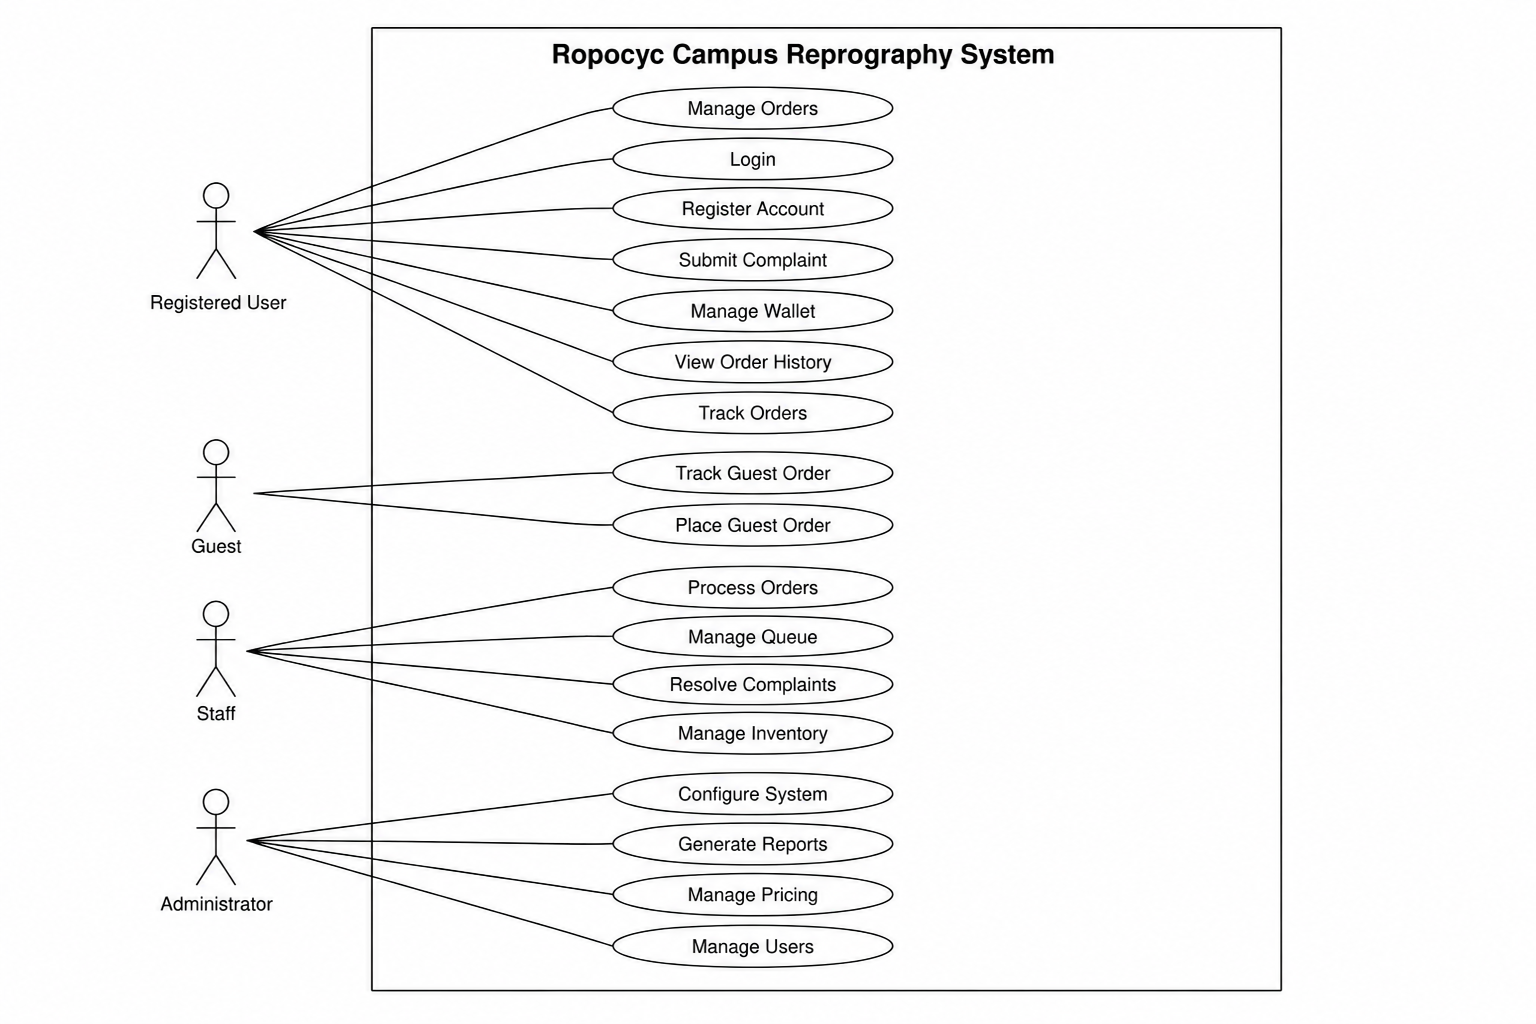
\includegraphics[width=0.85\textwidth,keepaspectratio]{figures/use_case_diagram.png}
\caption{Use Case Diagram}
\label{fig:use_case}
\end{figure}

% =========================================================================
% CHAPTER 4: SYSTEM DESIGN (EXACT SAMPLE PDF STRUCTURE)
% =========================================================================
\newpage
\chapter{SYSTEM DESIGN}

\section{4.1 Module Description}
The Reprography Automation System is structured into several interconnected modules, each responsible for specific operational functionality. The system follows a modular architecture to ensure maintainability, scalability, and clear separation of concerns.

\subsection{4.1.1 User Authentication Module}
This module handles user registration, login, and secure session management for students, faculty, and administrative staff using JSON Web Tokens (JWT) and bcrypt password hashing.
\begin{itemize}[leftmargin=0.35in, itemsep=1pt]
  \item \textbf{Input:} User credentials (name, email, password, role, department)
  \item \textbf{Output:} Authenticated user profile, signed JWT stored in httpOnly cookie
  \item \textbf{Description:} Validates institutional email domains, hashes passwords with salt factor 12, enforces role-based route access, and manages password reset tokens.
\end{itemize}

\subsection{4.1.2 Document Upload and Analysis Module}
This module captures uploaded files, validates MIME types, streams documents to Cloudinary, and extracts structural metrics for pre-flight verification.
\begin{itemize}[leftmargin=0.35in, itemsep=1pt]
  \item \textbf{Input:} PDF, DOCX, PNG, or JPEG file stream
  \item \textbf{Output:} Page count, color page count, blank page array, Cloudinary URL
  \item \textbf{Description:} Performs server-side buffer validation to reject non-document formats, computes page counts using pdf-lib, and detects blank pages to alert users.
\end{itemize}

\subsection{4.1.3 Order Configuration Wizard Module}
This module guides the customer through a step-by-step progress stepper to configure physical print options.
\begin{itemize}[leftmargin=0.35in, itemsep=1pt]
  \item \textbf{Input:} Copies, color mode, sidedness (duplex), paper size, binding type
  \item \textbf{Output:} Validated print specification object attached to pending order
  \item \textbf{Description:} Provides an interactive UI showing live visual previews and configuration summaries with paper conservation incentives.
\end{itemize}

\subsection{4.1.4 Dynamic Cost Estimation Module}
This module computes exact order tariffs in real time based on active institutional rates.
\begin{itemize}[leftmargin=0.35in, itemsep=1pt]
  \item \textbf{Input:} Page count, copies, color mode, duplex mode, binding selection
  \item \textbf{Output:} Total calculated price breakdown with applied discounts
  \item \textbf{Description:} Applies unit rates (B/W: INR 1.50, Color: INR 8.00), applies 0.85 multiplier discount for double-sided printing, and adds binding fees.
\end{itemize}

\subsection{4.1.5 Payment and Digital Wallet Module}
This module manages multi-channel payments, including Razorpay online transactions, internal student digital wallets, and cash-at-counter collections.
\begin{itemize}[leftmargin=0.35in, itemsep=1pt]
  \item \textbf{Input:} Payment method selection, wallet PIN or Razorpay signature
  \item \textbf{Output:} Verified payment transaction record, updated order paymentStatus
  \item \textbf{Description:} Executes atomic wallet deductions using MongoDB sessions, validates Razorpay webhook HMAC signatures, and manages Pay at Counter workflows.
\end{itemize}

\subsection{4.1.6 Composite Priority Queue Module}
This module organizes and sorts active orders in the production queue using a multi-factor priority algorithm.
\begin{itemize}[leftmargin=0.35in, itemsep=1pt]
  \item \textbf{Input:} Active orders in \texttt{In\_Queue} status with role, job size, and creation date
  \item \textbf{Output:} Ordered queue array with dynamic position numbers and estimated wait times
  \item \textbf{Description:} Evaluates effective priority scores by deducting 20 points for every full hour an order waits, eliminating queue starvation.
\end{itemize}

\subsection{4.1.7 Counter Staff Operations Module}
This module provides counter operators with a dedicated terminal to manage physical printing, cash settlements, and status transitions.
\begin{itemize}[leftmargin=0.35in, itemsep=1pt]
  \item \textbf{Input:} Staff action triggers (start processing, record cash, dispatch print)
  \item \textbf{Output:} Updated order status broadcasted via WebSockets to connected clients
  \item \textbf{Description:} Enables counter operators to advance orders through \texttt{Processing} and \texttt{ReadyForPickup} states and balance daily cash registers.
\end{itemize}

\subsection{4.1.8 OTP Pickup Handover Module}
This module enforces secure two-factor physical handover of finished printouts at the counter.
\begin{itemize}[leftmargin=0.35in, itemsep=1pt]
  \item \textbf{Input:} 4-digit pickup OTP entered by counter staff or QR-code scan
  \item \textbf{Output:} Order completion confirmation and digital handover timestamp
  \item \textbf{Description:} Verifies that the entered code matches the encrypted order secret before transitioning order to \texttt{Completed}.
\end{itemize}

\subsection{4.1.9 Administrator Governance Module}
This module serves as the central command center for institutional supervisors to manage platform settings.
\begin{itemize}[leftmargin=0.35in, itemsep=1pt]
  \item \textbf{Input:} Pricing updates, user role assignments, shop schedule modes
  \item \textbf{Output:} SystemConfig updates, exportable audit reports, activity logs
  \item \textbf{Description:} Enables dynamic rate adjustments, monitors system logs, and controls operating hours.
\end{itemize}

\subsection{4.1.10 Consumable Inventory Tracker Module}
This module tracks physical reprography supplies including paper reams, toner cartridges, and binding coils.
\begin{itemize}[leftmargin=0.35in, itemsep=1pt]
  \item \textbf{Input:} Stock additions, automated order page-count consumption
  \item \textbf{Output:} Real-time stock counts and low-inventory warning alerts
  \item \textbf{Description:} Decrements paper stock automatically upon order completion and alerts administrators when reorder thresholds are reached.
\end{itemize}

\subsection{4.1.11 Desktop Print Agent Module}
This module connects cloud queues to physical hardware installed on counter workstations.
\begin{itemize}[leftmargin=0.35in, itemsep=1pt]
  \item \textbf{Input:} Socket.IO print dispatch payload, signed document URL
  \item \textbf{Output:} Spooled physical print job, execution status telemetry
  \item \textbf{Description:} Discovers Windows printers using PowerShell, downloads files securely, and spools jobs directly to the printer driver.
\end{itemize}

\section{4.2 Schema Design}

\subsection{4.2.1 Database Tables}

\begin{table}[H]
\centering
\small
\caption{Users Table}
\label{tab:users}
\begin{tabular}{|p{1.2in}|p{1.2in}|p{3.2in}|}
\hline
\textbf{Field} & \textbf{Data Type} & \textbf{Description} \\ \hline
id & ObjectId & Unique identifier for each user (Primary Key) \\ \hline
name & String & User's full name \\ \hline
email & String & Institutional email address (unique) \\ \hline
password & String & Salted bcrypt password hash \\ \hline
role & String & Role classification (Student, Faculty, Staff, Admin) \\ \hline
department & String & Academic department \\ \hline
walletBalance & Number & Current pre-funded digital wallet balance \\ \hline
isVerified & Boolean & Email verification status flag \\ \hline
\end{tabular}
\end{table}

\begin{table}[H]
\centering
\small
\caption{Orders Table}
\label{tab:orders}
\begin{tabular}{|p{1.2in}|p{1.2in}|p{3.2in}|}
\hline
\textbf{Field} & \textbf{Data Type} & \textbf{Description} \\ \hline
id & ObjectId & Unique identifier for each order (Primary Key) \\ \hline
orderNumber & String & Human-readable tracking identifier (e.g. ORD-10024) \\ \hline
userId & ObjectId & Foreign key reference to Users collection \\ \hline
serviceType & String & Service category (Printing, Copy, Scan, Binding) \\ \hline
totalCost & Number & Total price in INR \\ \hline
paymentStatus & String & Settlement status (Pending, Paid, Cash\_Pending) \\ \hline
status & String & Order state (Pending, In\_Queue, Processing, Ready, Completed) \\ \hline
priorityScore & Number & Composite score governing queue position \\ \hline
pickupOtp & String & 4-digit secret code for handover verification \\ \hline
createdAt & DateTime & Order placement timestamp \\ \hline
\end{tabular}
\end{table}

\begin{table}[H]
\centering
\small
\caption{Documents Table}
\label{tab:documents}
\begin{tabular}{|p{1.2in}|p{1.2in}|p{3.2in}|}
\hline
\textbf{Field} & \textbf{Data Type} & \textbf{Description} \\ \hline
id & ObjectId & Unique identifier for document record (PK) \\ \hline
orderId & ObjectId & Foreign key linking to Orders collection \\ \hline
fileName & String & Original client file name \\ \hline
fileUrl & String & Secure signed cloud storage URL \\ \hline
pageCount & Number & Total verified pages in document \\ \hline
colorPages & Number & Count of pages containing color elements \\ \hline
fileSize & Number & Document size in bytes \\ \hline
\end{tabular}
\end{table}

\begin{table}[H]
\centering
\small
\caption{Payments Table}
\label{tab:payments}
\begin{tabular}{|p{1.2in}|p{1.2in}|p{3.2in}|}
\hline
\textbf{Field} & \textbf{Data Type} & \textbf{Description} \\ \hline
id & ObjectId & Unique payment identifier (PK) \\ \hline
orderId & ObjectId & Foreign key reference to Orders collection \\ \hline
userId & ObjectId & Foreign key reference to Users collection \\ \hline
amount & Number & Amount settled in INR \\ \hline
method & String & Payment channel (Razorpay, Wallet, Cash) \\ \hline
transactionId & String & Gateway transaction reference ID \\ \hline
status & String & Settlement status (Completed, Failed, Pending) \\ \hline
\end{tabular}
\end{table}

\subsection{4.2.2 Relationships}
\begin{itemize}[leftmargin=0.35in, itemsep=2pt]
  \item \textbf{users $\rightarrow$ orders:} one-to-many (each user can place multiple orders)
  \item \textbf{orders $\rightarrow$ documents:} one-to-many (each order can contain multiple document files)
  \item \textbf{orders $\rightarrow$ payments:} one-to-one (each order is associated with exactly one payment record)
  \item \textbf{users $\rightarrow$ wallet:} one-to-one (each user owns exactly one digital wallet balance)
  \item \textbf{agents $\rightarrow$ print\_jobs:} one-to-many (each print agent spools multiple assigned jobs)
\end{itemize}

\subsection{4.2.3 Constraints}
\begin{itemize}[leftmargin=0.35in, itemsep=2pt]
  \item Primary key indexes enforce absolute record uniqueness across all collections.
  \item Foreign key object references maintain referential integrity across users, orders, and documents.
  \item Not null constraints are enforced on essential transaction fields (amounts, statuses, hashes).
  \item Default values guarantee deterministic system behavior when optional parameters are omitted.
\end{itemize}

\section{4.3 Procedural/Flow Design}

\subsection{4.3.1 Order and Production Flowchart}
This flowchart represents the step-by-step process of placing and processing an order:
\begin{itemize}[leftmargin=0.35in, itemsep=2pt]
  \item User logs into portal or kiosk terminal
  \item User uploads document file(s) $\rightarrow$ pdf-lib extracts page counts and inspects blank pages
  \item User selects print parameters (copies, color, duplex, binding)
  \item System computes deterministic cost quotation
  \item User selects payment method:
    \begin{itemize}
      \item If Wallet $\rightarrow$ Atomic balance debit $\rightarrow$ Status: \texttt{In\_Queue}
      \item If Razorpay $\rightarrow$ Complete online payment $\rightarrow$ Webhook verifies $\rightarrow$ Status: \texttt{In\_Queue}
      \item If Cash at Counter $\rightarrow$ Status: \texttt{In\_Queue}, Payment: \texttt{Cash\_Pending}
    \end{itemize}
  \item Priority queue engine evaluates base priority and dynamic aging deduction
  \item Staff dashboard displays order; operator prints output via Desktop Print Agent
  \item Operator transitions order to \texttt{ReadyForPickup} $\rightarrow$ Customer receives notification and 4-digit OTP
  \item Customer presents OTP at counter $\rightarrow$ Staff enters OTP $\rightarrow$ Order marked \texttt{Completed}
\end{itemize}

\begin{figure}[H]
\centering
\begin{tikzpicture}[node distance=1.3cm, auto,
  block/.style={rectangle, draw, fill=blue!5, text width=2.6in, text centered, rounded corners, minimum height=0.35in, font=\footnotesize},
  decision/.style={diamond, draw, fill=yellow!10, text width=1.4in, text centered, font=\tiny},
  line/.style={draw, -{Latex[length=2mm]}, thick}]
  
  \node [block] (step1) {User Uploads Document \& Configures Options};
  \node [block, below of=step1] (step2) {Pre-Flight Analysis Extracts Pages \& Estimates Cost};
  \node [decision, below of=step2, yshift=-0.2cm] (pay) {Select Payment Method};
  \node [block, left of=pay, xshift=-1.6cm] (wallet) {Wallet: Atomic Debit};
  \node [block, right of=pay, xshift=1.6cm] (online) {Razorpay: Online Gateway};
  \node [block, below of=pay, yshift=-0.5cm] (queue) {Priority Queue Placement with Aging};
  \node [block, below of=queue] (print) {Staff / Print Agent Spools Output};
  \node [block, below of=print] (pickup) {OTP Handover Verification at Counter};
  
  \path [line] (step1) -- (step2);
  \path [line] (step2) -- (pay);
  \path [line] (pay) -| (wallet);
  \path [line] (pay) -| (online);
  \path [line] (wallet) |- (queue);
  \path [line] (online) |- (queue);
  \path [line] (pay) -- node[right, font=\tiny]{Cash} (queue);
  \path [line] (queue) -- (print);
  \path [line] (print) -- (pickup);
\end{tikzpicture}
\caption{Order Placement and Production Flowchart}
\label{fig:order_flowchart}
\end{figure}

\section{4.4 User Interface Design}
User Interface Design is the visual and interactive component of a system through which users interact with it. In the Reprography Automation System, the UI has been carefully designed for two types of users: customers (students/faculty/guests) and administrators/staff.

\subsection{4.4.1 Client Interface}
\begin{itemize}[leftmargin=0.35in, itemsep=2pt]
  \item \textbf{Landing and Upload Portal:} Clean file dropzone with real-time format detection and pre-flight analysis cards.
  \item \textbf{Configuration Wizard Stepper:} Responsive 3-step progress stepper with live cost computation and coupon redemption inputs.
  \item \textbf{Order Status Timeline:} Visual progress timeline displaying real-time position badges, countdown timers, and pickup OTP cards.
  \item \textbf{Digital Wallet Card:} Live balance display, quick recharge buttons, and chronological transaction history.
\end{itemize}

\subsection{4.4.2 Administrator and Staff Interface}
\begin{itemize}[leftmargin=0.35in, itemsep=2pt]
  \item \textbf{Staff Production Queue:} Real-time queue board grouping active orders by service category with single-click status update triggers and cash verification buttons.
  \item \textbf{OTP Verification Modal:} Secure numeric modal requiring entry of the customer's 4-digit code before releasing output.
  \item \textbf{Admin Governance Console:} Real-time statistics, tariff configuration tables, consumable stock monitors, and exportable financial audit logs.
\end{itemize}

% =========================================================================
% CHAPTER 5: AGILE METHODOLOGY (EXACT SAMPLE PDF STRUCTURE)
% =========================================================================
\newpage
\chapter{AGILE METHODOLOGY}

\section{5.1 Project Roadmap}
The development of the Reprography Automation System followed an Agile roadmap structured across weekly sprint increments, as detailed in Table 5.1.

\begin{table}[H]
\centering
\small
\caption{Project Roadmap}
\label{tab:roadmap}
\begin{tabular}{|p{0.8in}|p{4.6in}|}
\hline
\textbf{Week} & \textbf{Tasks Completed} \\ \hline
Week 1 & Finalized project topic and scope. Scrum Master divided requirements into task units. \\ \hline
Week 2 & Created Git repository. Started designing user registration form and dashboard wireframes. \\ \hline
Week 3 & Improved UI of order wizard and dashboard. Created authentication views for students and staff. \\ \hline
Week 4 & Implemented document upload pipeline and PDF parsing module for page counts. \\ \hline
Week 5 & Created MongoDB schemas for users, orders, and documents. Enhanced upload UI. \\ \hline
Week 6 & Completed first project review with guide feedback and architectural refinement. \\ \hline
Week 7 & Developed staff queue dashboard, order status transitions, and cash payment recording. \\ \hline
Week 8 & Created dynamic pricing service and anti-starvation priority queue engine. \\ \hline
Week 9 & Integrated Razorpay payment gateway and ACID-compliant student digital wallet. \\ \hline
Week 10 & Implemented OTP pickup verification at counter and real-time Socket.IO synchronization. \\ \hline
Week 11 & Developed administrator console for tariff management, inventory tracking, and audit logs. \\ \hline
Week 12 & Built autonomous Electron desktop Print Agent with Windows spooler integration. \\ \hline
Week 13 & Added background shop scheduling cron services (09:00 to 17:00 IST) and order timeouts. \\ \hline
Week 14 & Implemented Progressive Web App (PWA) service worker caching and Web Push notifications. \\ \hline
Week 15 & Executed automated Selenium test suite across 120 test cases and resolved edge cases. \\ \hline
Week 16 & Completed final UI polish, system deployment on cloud servers, and report documentation. \\ \hline
\end{tabular}
\end{table}

\section{5.2 User Stories}
In the Agile development process, the project was divided into multiple user stories, each representing a real-world requirement from the perspective of a specific stakeholder persona.

\subsection{5.2.1 User Stories}
\noindent\textbf{Student}
\begin{itemize}[leftmargin=0.35in, itemsep=2pt]
  \item As a student, I want to upload my assignment PDF from my phone so that I do not have to wait in the physical counter queue.
  \item As a student, I want to see an instant price breakdown before paying so that I know exactly how much the print job will cost.
  \item As a student, I want to pay using UPI or my college wallet so that I do not need exact cash currency.
  \item As a student, I want to track my order status in real time so that I know exactly when to walk to the counter for collection.
  \item As a student, I want to receive an OTP code so that my documents cannot be collected by unauthorized persons.
\end{itemize}

\noindent\textbf{Faculty / Staff / Admin}
\begin{itemize}[leftmargin=0.35in, itemsep=2pt]
  \item As a faculty member, I want my urgent exam question papers to receive prioritized counter processing to meet submission deadlines.
  \item As a counter staff operator, I want to see incoming jobs sorted by priority so that I can print urgent and long-waiting jobs efficiently.
  \item As a counter staff operator, I want to verify a 4-digit OTP before handing over prints so that jobs are never misplaced.
  \item As an administrator, I want to update per-page print tariffs live so that prices reflect changes in institutional paper costs.
  \item As an administrator, I want to track consumable inventory (paper reams, toner) so that the shop never runs out of essential stock.
\end{itemize}

\subsection{5.2.2 Sprint Planning}
Each sprint focused on a functional module or major architectural subsystem. The sprint goals were planned as follows:

\begin{table}[H]
\centering
\small
\caption{Sprint Planning Table}
\label{tab:sprint}
\begin{tabular}{|p{0.8in}|p{4.6in}|}
\hline
\textbf{Sprint} & \textbf{Key Activities / Focus} \\ \hline
Sprint 1 & Requirement gathering, system feasibility, and task distribution by the Scrum Master. \\ \hline
Sprint 2 & Design and prototyping of the responsive order wizard and dashboard interfaces. \\ \hline
Sprint 3 & Implementation of JWT authentication, role guards, and profile management. \\ \hline
Sprint 4 & Development of file upload pipeline, Cloudinary integration, and PDF pre-flight checks. \\ \hline
Sprint 5 & Database creation in MongoDB Atlas and ACID wallet transaction implementation. \\ \hline
Sprint 6 & First project review and architectural feedback adjustments. \\ \hline
Sprint 7 & Priority queue algorithm implementation with dynamic aging deduction functions. \\ \hline
Sprint 8 & Staff production dashboard development and cash-at-counter settlement controls. \\ \hline
Sprint 9--11 & Razorpay gateway integration, Socket.IO real-time engine, and Electron Print Agent. \\ \hline
Sprint 12--14 & Automated shop scheduler cron, OTP verification, PWA service worker, and inventory tracker. \\ \hline
Sprint 15--16 & Automated Selenium test suite execution, bug fixes, deployment, and final documentation. \\ \hline
\end{tabular}
\end{table}

\section{5.3 Test Plan}
The testing phase was designed to ensure that the Reprography Automation System works reliably, securely, and as intended. The main objective was to validate that each module performs its specific function correctly, both individually and when integrated into the complete platform.

The test plan followed incremental and iterative principles consistent with Agile methodology. Modules were tested after development in small cycles, allowing early detection and resolution of errors:
\begin{itemize}[leftmargin=0.35in, itemsep=2pt]
  \item \textbf{Functional Accuracy:} Ensuring all features such as document upload, page counting, pricing, priority sorting, OTP validation, and print spooling function correctly.
  \item \textbf{Integration Reliability:} Verifying that all modules---React frontend, Express backend, MongoDB Atlas, Cloudinary, Razorpay, Socket.IO, and Electron Print Agent---communicate without errors.
  \item \textbf{Security and Data Integrity:} Checking that user passwords, JWT sessions, OTP codes, and financial wallet transactions are securely processed and stored.
  \item \textbf{Error Handling:} Ensuring the system gracefully handles invalid file types, expired sessions, payment cancellations, and printer spooler disconnects.
  \item \textbf{Usability:} Assessing the ease of use of the order wizard, staff dashboard, and kiosk interface for real-world campus scenarios.
\end{itemize}

% =========================================================================
% CHAPTER 6: IMPLEMENTATION AND TESTING (EXACT SAMPLE PDF STRUCTURE)
% =========================================================================
\newpage
\chapter{IMPLEMENTATION AND TESTING}

\section{6.1 Implementation Procedures}
The implementation of the Reprography Automation System was carried out in modular steps, combining the React frontend, Express.js backend, MongoDB database, Socket.IO real-time engine, and native Electron Print Agent:

\noindent\textbf{Step 1: Development Environment Setup}
\begin{itemize}[leftmargin=0.35in, itemsep=1pt]
  \item Node.js and Express framework configured for backend API routing.
  \item MongoDB Atlas database initialized with connection pooling and Mongoose schemas.
  \item Vite and React 19 environment set up with Tailwind CSS for modern responsive styling.
\end{itemize}

\noindent\textbf{Step 2: Client Order Wizard Interface}
\begin{itemize}[leftmargin=0.35in, itemsep=1pt]
  \item Multi-step wizard implemented for document upload, parameter selection, and checkout.
  \item Client-side file pre-flight inspection incorporated using pdf-lib and pdfjs-dist.
  \item Dynamic price calculation with automatic 15\% duplex discount applied in real time.
\end{itemize}

\noindent\textbf{Step 3: Document Processing and Storage Pipeline}
\begin{itemize}[leftmargin=0.35in, itemsep=1pt]
  \item Multer memory storage configured with MIME validation to block executable file uploads.
  \item Stream-based upload to Cloudinary implemented, returning secure, signed URLs.
  \item Server-side page counting and blank-page detection executed during file intake.
\end{itemize}

\noindent\textbf{Step 4: Priority Queue and Pricing Services}
\begin{itemize}[leftmargin=0.35in, itemsep=1pt]
  \item Dynamic priority scoring service implemented combining role weights and estimated job durations.
  \item Anti-starvation aging algorithm added, reducing queue score by 20 points for each full waiting hour.
  \item Multi-channel payment engine constructed supporting Razorpay, ACID wallet debits, and PAC cash.
\end{itemize}

\noindent\textbf{Step 5: Staff Counter and Admin Dashboards}
\begin{itemize}[leftmargin=0.35in, itemsep=1pt]
  \item Real-time queue board developed displaying active orders sorted by effective priority.
  \item Single-click production controls implemented for cash verification and status transitions.
  \item Administrative console built for live tariff adjustments, inventory tracking, and audit logging.
\end{itemize}

\noindent\textbf{Step 6: Hardware Interfacing and Automation}
\begin{itemize}[leftmargin=0.35in, itemsep=1pt]
  \item Electron desktop Print Agent developed to bridge cloud queues to local Windows printers.
  \item Windows PowerShell integration implemented for local printer discovery and heartbeat reporting.
  \item Background automated spooling executed via pdf-to-printer upon Socket.IO dispatch.
\end{itemize}

\noindent\textbf{Step 7: Automated Scheduling and PWA Finalization}
\begin{itemize}[leftmargin=0.35in, itemsep=1pt]
  \item node-cron service configured to enforce institutional hours (09:00 to 17:00 IST) and Sunday closures.
  \item Service worker and web app manifest configured for PWA installation and offline caching.
  \item End-to-end automated testing executed using Python Selenium WebDriver.
\end{itemize}

\section{6.2 Testing Methods and Results}
The testing phase aimed to verify the functionality, reliability, and security of the Reprography Automation System. Testing was carried out incrementally as each module was developed, following Agile methodology.

\subsection{6.2.1 Unit Testing}
Each individual module (pricing calculation, aging deduction, JWT verification, OTP generation, MIME validation) was tested in isolation to ensure correct algorithmic accuracy.

\subsection{6.2.2 Integration Testing}
Combined operations such as document upload $\rightarrow$ Cloudinary storage $\rightarrow$ cost estimation $\rightarrow$ Razorpay webhook $\rightarrow$ queue insertion $\rightarrow$ Socket.IO broadcast were rigorously tested to ensure smooth data flow.

\subsection{6.2.3 System Testing}
The complete system, including the React web client, Express backend, MongoDB database, staff dashboard, and Electron desktop Print Agent, was tested under simulated peak submission workloads.

\subsection{6.2.4 User Acceptance Testing}
Sample student users and reprography operators tested the system in realistic campus scenarios to evaluate usability, responsiveness, and satisfaction with real-world workflows.

\noindent\textbf{Key Test Scenarios and Results} \\
\noindent\textit{Authentication and Access Control:}
\begin{itemize}[leftmargin=0.35in, itemsep=1pt]
  \item Valid login credentials successfully returned JWT token in httpOnly cookie.
  \item Protected staff and admin routes correctly blocked unauthorized student access with 403 Forbidden.
\end{itemize}

\noindent\textit{Document Upload and Pricing:}
\begin{itemize}[leftmargin=0.35in, itemsep=1pt]
  \item PDF page counts were extracted with 100\% accuracy across single and multi-page test documents.
  \item Double-sided discount (0.85 multiplier) and binding tariffs were computed correctly.
\end{itemize}

\noindent\textit{Payment and Queue Operations:}
\begin{itemize}[leftmargin=0.35in, itemsep=1pt]
  \item Digital wallet payments executed atomically using MongoDB sessions without double-deduction risks.
  \item Orders waiting over 60 minutes received automated 20-point aging deductions, advancing queue rank.
\end{itemize}

\noindent\textit{OTP Handover and Hardware Spooling:}
\begin{itemize}[leftmargin=0.35in, itemsep=1pt]
  \item Valid 4-digit pickup OTPs successfully transitioned orders to Completed; incorrect OTPs were rejected.
  \item Desktop Print Agent successfully received Socket.IO dispatch payloads and spooled test PDFs.
\end{itemize}

\noindent\textbf{Security and Error Handling}
\begin{itemize}[leftmargin=0.35in, itemsep=1pt]
  \item Non-document executable (.exe) uploads were blocked by MIME inspection.
  \item Rate-limiting middleware successfully prevented API brute-force attempts.
\end{itemize}

\noindent\textbf{Outcome}
\begin{itemize}[leftmargin=0.35in, itemsep=1pt]
  \item 114 out of 120 automated Selenium test cases passed successfully (95.0\% pass rate).
  \item The system demonstrated stable, accurate, and secure operation, providing a reliable and user-friendly reprography automation solution.
\end{itemize}

% =========================================================================
% CHAPTER 7: CONCLUSIONS (EXACT SAMPLE PDF STRUCTURE)
% =========================================================================
\newpage
\chapter{CONCLUSIONS}

\section{7.1 Summary}
The Reprography Automation System (REPOSYS) was developed to overcome the limitations of traditional manual campus reprography methods. The system integrates a modern responsive web client, an Express.js backend, a MongoDB Atlas database, real-time WebSockets, and a native Electron desktop Print Agent to provide automated, secure, and efficient document printing management.

Key features include:
\begin{itemize}[leftmargin=0.35in, itemsep=2pt]
  \item Pre-flight document analysis and automated page-count extraction.
  \item Multi-channel payment processing via Razorpay, digital wallet, and Pay at Counter.
  \item Composite priority queue with dynamic aging deduction to guarantee student fairness.
  \item Secure OTP and QR-code handover verification at the counter.
  \item Real-time operational transparency via Socket.IO event broadcasting.
  \item Autonomous hardware print spooling via desktop Print Agent.
  \item Automated institutional shop scheduling (09:00 to 17:00 IST) and timeout management.
\end{itemize}
The system significantly reduces physical lobby queues, protects student document privacy, prevents billing errors, and ensures accurate, traceable records of every transaction. The project demonstrates the successful integration of modern web technologies, real-time messaging, and desktop automation for practical, real-world academic applications.

\section{7.2 Limitations}
\begin{itemize}[leftmargin=0.35in, itemsep=2pt]
  \item Very large document uploads (>100 MB) can experience latency on slow mobile networks.
  \item Free serverless cloud tiers introduce cold-start response delays upon initial wake-up.
  \item The Print Agent currently relies on Windows Print Spooler APIs, requiring Windows-based counter PCs.
  \item Uncollected Pay at Counter orders printed prior to cash collection remain a minor financial risk.
\end{itemize}

\section{7.3 Future Scope}
\begin{itemize}[leftmargin=0.35in, itemsep=2pt]
  \item \textbf{Native Mobile Applications:} Develop native iOS and Android apps using React Native with push notifications.
  \item \textbf{Smart Campus RFID Card Integration:} Enable students to tap their institutional ID cards for instant authentication and payment.
  \item \textbf{AI Document Intelligence:} Integrate Google Gemini API for automated font legibility checks, multi-language translation, and document summarization.
  \item \textbf{Multi-Shop Load Balancing:} Distribute printing workloads dynamically across multiple departmental print centres based on queue congestion.
  \item \textbf{Self-Service Hardware Kiosks:} Deploy unattended kiosks equipped with cash acceptors and automated output sorting trays for 24/7 service.
\end{itemize}

% =========================================================================
% CHAPTER 8: APPENDICES (EXACT SAMPLE PDF STRUCTURE)
% =========================================================================
\newpage
\chapter{APPENDICES}

\section{8.1 Code}

\noindent\textbf{8.1.1 index.html (Client Order Form \& Kiosk)}
\begin{lstlisting}[language=html]
<!DOCTYPE html>
<html lang="en">
<head>
  <meta charset="UTF-8">
  <title>REPOSYS - Campus Reprography</title>
  <link rel="stylesheet" href="/styles/main.css">
</head>
<body class="bg-slate-900 text-white min-h-screen">
  <div class="container mx-auto px-4 py-8">
    <header class="flex justify-between items-center mb-8">
      <div class="flex items-center gap-3">
        <img src="/assets/logo.png" alt="REPOSYS Logo" class="h-10">
        <h1 class="text-2xl font-bold">REPOSYS</h1>
      </div>
      <div id="userBadge" class="flex items-center gap-2">
        <span id="userName" class="text-sm font-medium">Guest User</span>
        <span id="walletBal" class="bg-blue-600 px-3 py-1 rounded-full text-xs">Bal: INR 0.00</span>
      </div>
    </header>

    <main class="max-w-2xl mx-auto bg-slate-800 p-6 rounded-xl shadow-xl">
      <div class="mb-6">
        <h2 class="text-xl font-bold mb-2">Upload Document</h2>
        <div id="dropzone" class="border-2 border-dashed border-slate-600 p-8 text-center rounded-lg cursor-pointer hover:border-blue-500">
          <input type="file" id="fileInput" class="hidden" accept=".pdf,.docx,.png,.jpg">
          <p class="text-slate-400">Drag & Drop PDF or Click to Browse</p>
        </div>
      </div>

      <div id="configSection" class="space-y-4 hidden">
        <div class="grid grid-cols-2 gap-4">
          <div>
            <label class="text-sm text-slate-300">Copies</label>
            <input type="number" id="copies" value="1" min="1" class="w-full bg-slate-700 rounded p-2 text-white">
          </div>
          <div>
            <label class="text-sm text-slate-300">Color Mode</label>
            <select id="colorMode" class="w-full bg-slate-700 rounded p-2 text-white">
              <option value="BlackAndWhite">Black & White (INR 1.50/page)</option>
              <option value="Color">Full Color (INR 8.00/page)</option>
            </select>
          </div>
        </div>

        <div class="grid grid-cols-2 gap-4">
          <div>
            <label class="text-sm text-slate-300">Duplex</label>
            <select id="sided" class="w-full bg-slate-700 rounded p-2 text-white">
              <option value="Single">Single-Sided</option>
              <option value="Double">Double-Sided (15% Paper Discount)</option>
            </select>
          </div>
          <div>
            <label class="text-sm text-slate-300">Binding</label>
            <select id="binding" class="w-full bg-slate-700 rounded p-2 text-white">
              <option value="None">None</option>
              <option value="Spiral">Spiral Binding (INR 100)</option>
            </select>
          </div>
        </div>

        <div class="bg-slate-700 p-4 rounded-lg flex justify-between items-center">
          <div>
            <span class="text-xs text-slate-400">Estimated Total</span>
            <p id="totalPrice" class="text-2xl font-bold text-green-400">INR 0.00</p>
          </div>
          <button id="checkoutBtn" class="bg-blue-600 hover:bg-blue-500 text-white px-6 py-2 rounded-lg font-bold">
            Proceed to Payment
          </button>
        </div>
      </div>
    </main>
  </div>
</body>
</html>
\end{lstlisting}

\noindent\textbf{8.1.2 queueService.js (Priority Queue \& Aging Implementation)}
\begin{lstlisting}[language=JavaScript]
const Order = require('../models/Order');
const socketHandler = require('../socket/socketHandler');
const { calculateEffectivePriority, calculateAgingDeduction } = require('./pricingService');

const VISIBLE_QUEUE_STATUSES = ['In_Queue', 'Processing', 'ReadyForPickup'];

const resolvePriorityScore = (order) => {
  const storedPriorityScore = Number(order.priorityScore);
  return Number.isFinite(storedPriorityScore) ? storedPriorityScore : 200;
};

const toQueueItem = (order, position) => {
  const baseScore = resolvePriorityScore(order);
  const effectivePriorityScore = calculateEffectivePriority(baseScore, order.createdAt);
  
  return {
    ...order.toObject(),
    priorityScore: effectivePriorityScore,
    basePriority: baseScore,
    agingDeduction: calculateAgingDeduction(order.createdAt),
    position,
  };
};

async function getQueue(serviceType) {
  const orders = await Order.find({
    serviceType,
    status: { $in: VISIBLE_QUEUE_STATUSES },
  })
    .populate('userId', 'name role department')
    .sort({ createdAt: 1 });

  return orders
    .map((order) => toQueueItem(order, 0))
    .sort((left, right) => {
      if (left.priorityScore !== right.priorityScore) {
        return left.priorityScore - right.priorityScore;
      }
      return new Date(left.createdAt).getTime() - new Date(right.createdAt).getTime();
    })
    .map((order, index) => ({
      ...order,
      position: index + 1,
    }));
}

async function broadcastQueueUpdate(serviceType) {
  const queue = await getQueue(serviceType);
  const io = socketHandler.getIO();

  io.to(`queue:${serviceType}`).emit('queue_update', {
    type: 'queue_update',
    serviceType,
    queue,
  });
}

module.exports = { getQueue, broadcastQueueUpdate };
\end{lstlisting}

\noindent\textbf{8.1.3 shopScheduler.js (Automated IST Shop Operating Hours)}
\begin{lstlisting}[language=JavaScript]
const cron = require('node-cron');
const SystemConfig = require('../models/SystemConfig');

const startShopScheduler = (io) => {
  cron.schedule('* * * * *', async () => {
    try {
      const now = new Date();
      const istOffset = 5.5 * 60 * 60 * 1000;
      const istTime = new Date(now.getTime() + istOffset);
      const hours = istTime.getUTCHours();
      const minutes = istTime.getUTCMinutes();
      const day = istTime.getUTCDay();

      const currentMinutes = hours * 60 + minutes;
      const openMinutes = 9 * 60;
      const closeMinutes = 17 * 60;

      const shouldBeOpen = day !== 0 &&
                           currentMinutes >= openMinutes &&
                           currentMinutes < closeMinutes;

      const config = await SystemConfig.getInstance();
      if (!config || config.shopMode !== 'schedule') return;

      if (config.isManuallyOpen === shouldBeOpen) return;

      config.isManuallyOpen = shouldBeOpen;
      await config.save();

      const eventName = shouldBeOpen ? 'shop_opened' : 'shop_closed';
      io.emit(eventName, { type: eventName });

      console.log(`[ShopScheduler] Shop ${shouldBeOpen ? 'opened' : 'closed'} at ${hours}:${minutes} IST`);
    } catch (err) {
      console.error('[ShopScheduler] Cron error:', err);
    }
  });
};

module.exports = { startShopScheduler };
\end{lstlisting}

\noindent\textbf{8.1.4 PrintAgent/main.js (Electron Native Windows Spooler)}
\begin{lstlisting}[language=JavaScript]
const { app, BrowserWindow, ipcMain, Tray, Menu } = require('electron');
const path = require('path');
const io = require('socket.io-client');
const ptp = require('pdf-to-printer');
const axios = require('axios');
const fs = require('fs');

let socket;
let mainWindow;

function initSocket(agentConfig) {
  socket = io(agentConfig.serverUrl, {
    auth: {
      agentId: agentConfig.agentId,
      agentSecret: agentConfig.agentSecret,
    },
  });

  socket.on('connect', () => {
    console.log('[PrintAgent] Connected to cloud dispatch server');
  });

  socket.on('print_dispatch', async (data) => {
    try {
      console.log(`[PrintAgent] Received print job #${data.orderNumber}`);
      const tempPath = path.join(app.getPath('temp'), `${data.orderNumber}.pdf`);
      
      const response = await axios({
        url: data.signedFileUrl,
        method: 'GET',
        responseType: 'stream',
      });
      
      const writer = fs.createWriteStream(tempPath);
      response.data.pipe(writer);

      writer.on('finish', async () => {
        await ptp.print(tempPath, {
          printer: data.targetPrinter || undefined,
        });
        socket.emit('job_status_update', {
          orderId: data.orderId,
          status: 'Printed',
        });
        fs.unlinkSync(tempPath);
      });
    } catch (err) {
      console.error('[PrintAgent] Spooler error:', err);
    }
  });
}
\end{lstlisting}

\noindent\textbf{8.1.5 walletController.js (ACID-Compliant Wallet Settlement)}
\begin{lstlisting}[language=JavaScript]
const mongoose = require('mongoose');
const User = require('../models/User');
const Order = require('../models/Order');
const Payment = require('../models/Payment');

exports.payWithWallet = async (req, res) => {
  const session = await mongoose.startSession();
  session.startTransaction();
  try {
    const { orderId } = req.body;
    const userId = req.user.id;

    const user = await User.findById(userId).session(session);
    const order = await Order.findById(orderId).session(session);

    if (!order || order.userId.toString() !== userId) {
      await session.abortTransaction();
      return res.status(404).json({ error: 'Order not found' });
    }

    if (user.walletBalance < order.totalCost) {
      await session.abortTransaction();
      return res.status(400).json({ error: 'Insufficient wallet balance' });
    }

    user.walletBalance -= order.totalCost;
    order.paymentStatus = 'Paid';
    order.paymentMethod = 'Wallet';
    order.status = 'In_Queue';

    await user.save({ session });
    await order.save({ session });

    await Payment.create([{
      orderId: order._id,
      userId: user._id,
      amount: order.totalCost,
      method: 'Wallet',
      status: 'Completed'
    }], { session });

    await session.commitTransaction();
    res.json({ success: true, balance: user.walletBalance });
  } catch (err) {
    await session.abortTransaction();
    res.status(500).json({ error: 'Transaction failed', details: err.message });
  } finally {
    session.endSession();
  }
};
\end{lstlisting}

\section{8.2 Screenshots}
The verified user interface views of the Reprography Automation System are presented below:

\newpage
\begin{figure}[H]
\centering

\includegraphics[width=0.85\textwidth,keepaspectratio]{figures/screen_home.png}
\caption{Public Landing and Portal Gateway}
\end{figure}
\vspace{0.3in}
\begin{figure}[H]
\centering
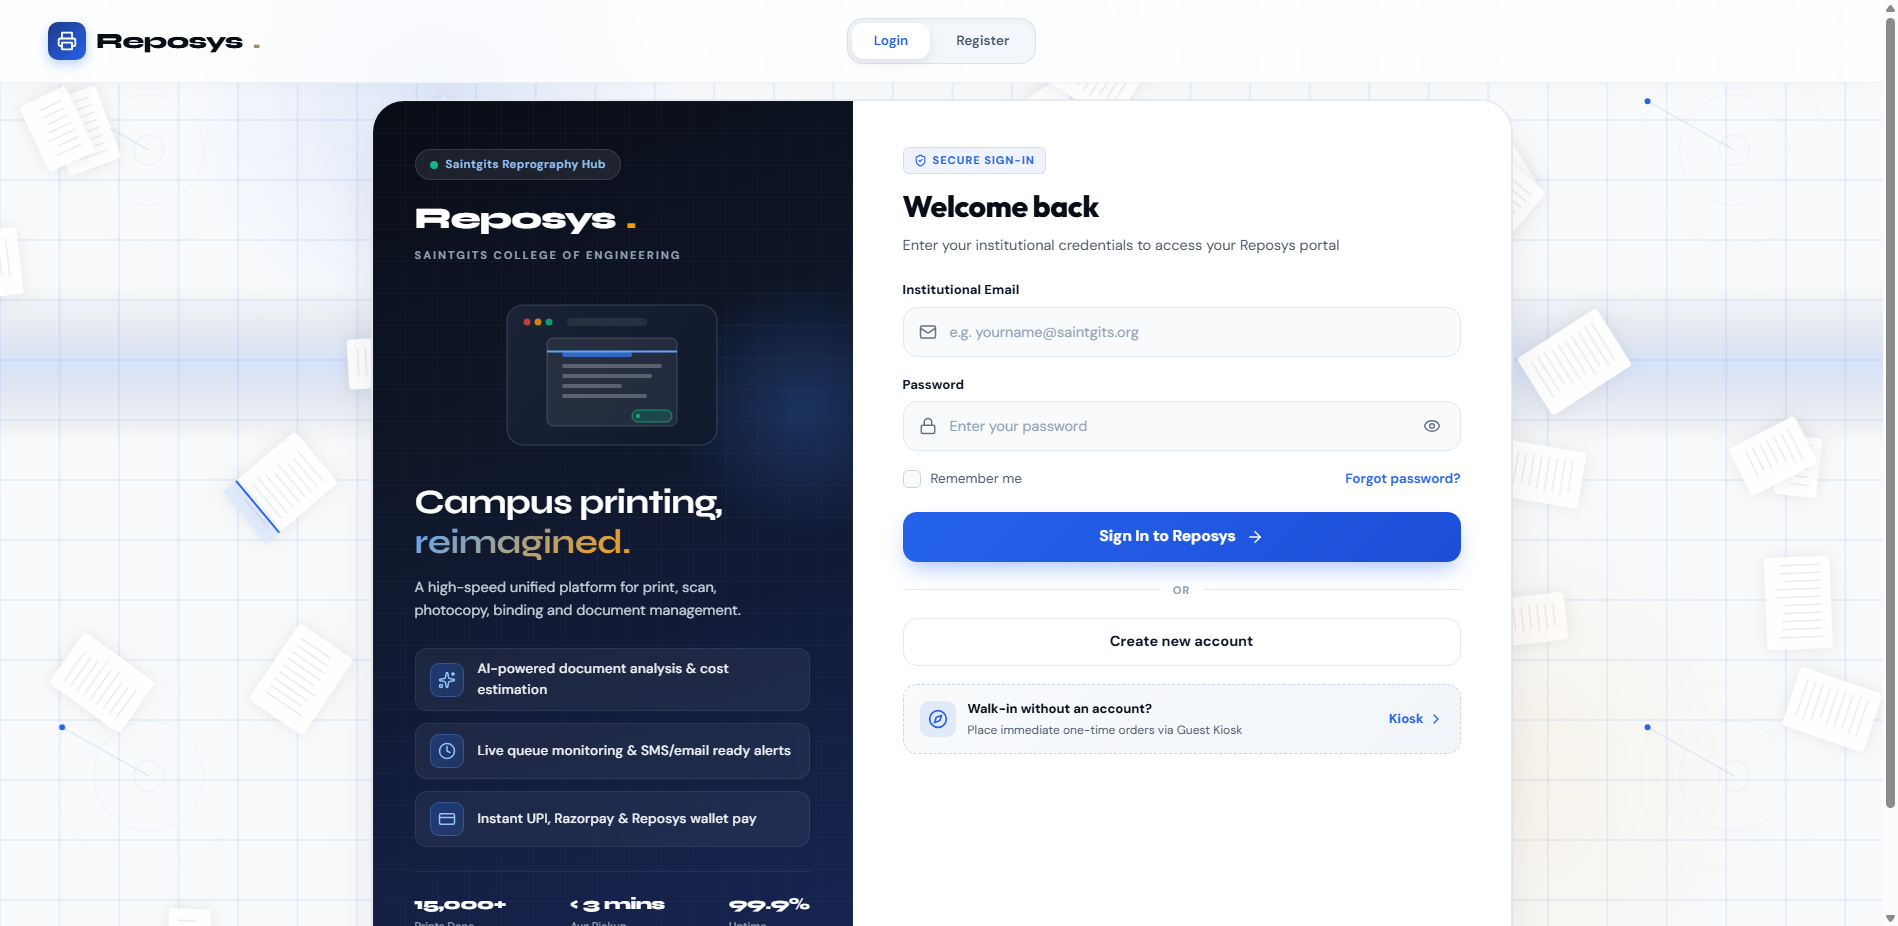
\includegraphics[width=0.85\textwidth,keepaspectratio]{figures/screen_login.png}
\caption{Secure User Authentication and Multi-Role Login Portal}
\end{figure}

\newpage
\begin{figure}[H]
\centering
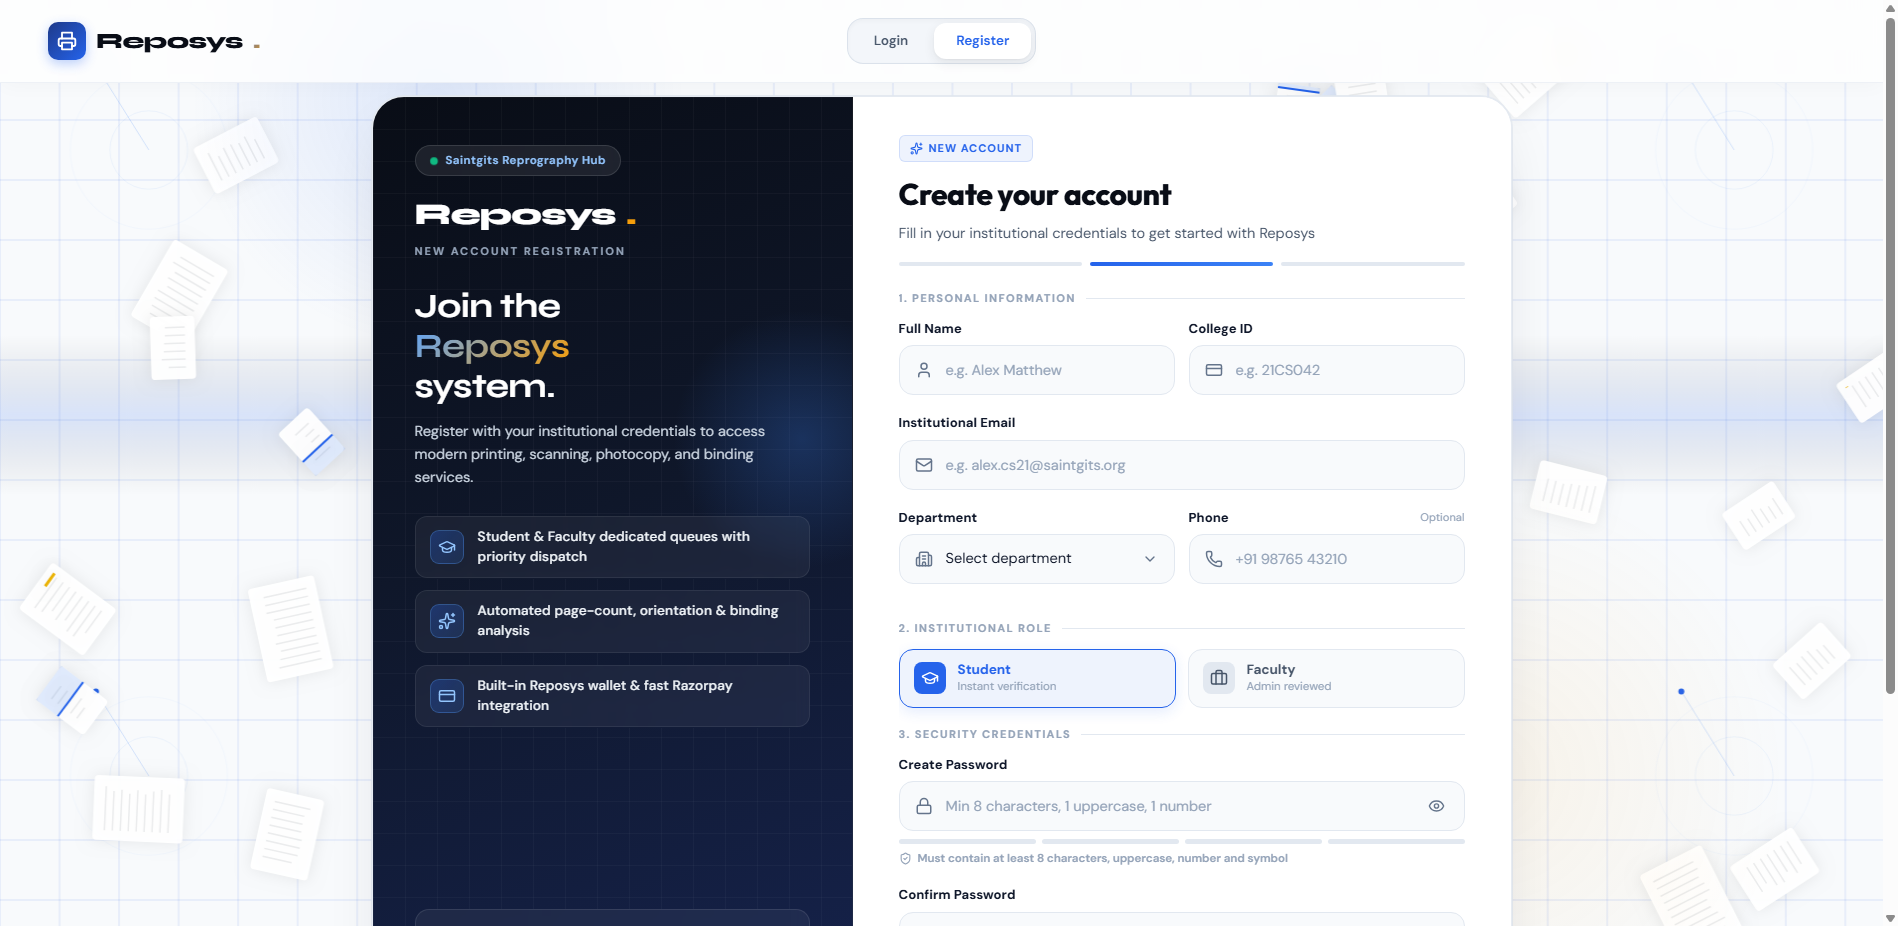
\includegraphics[width=0.85\textwidth,keepaspectratio]{figures/screen_register.png}
\caption{Account Registration Portal with Institutional Email Validation}
\end{figure}
\vspace{0.3in}
\begin{figure}[H]
\centering
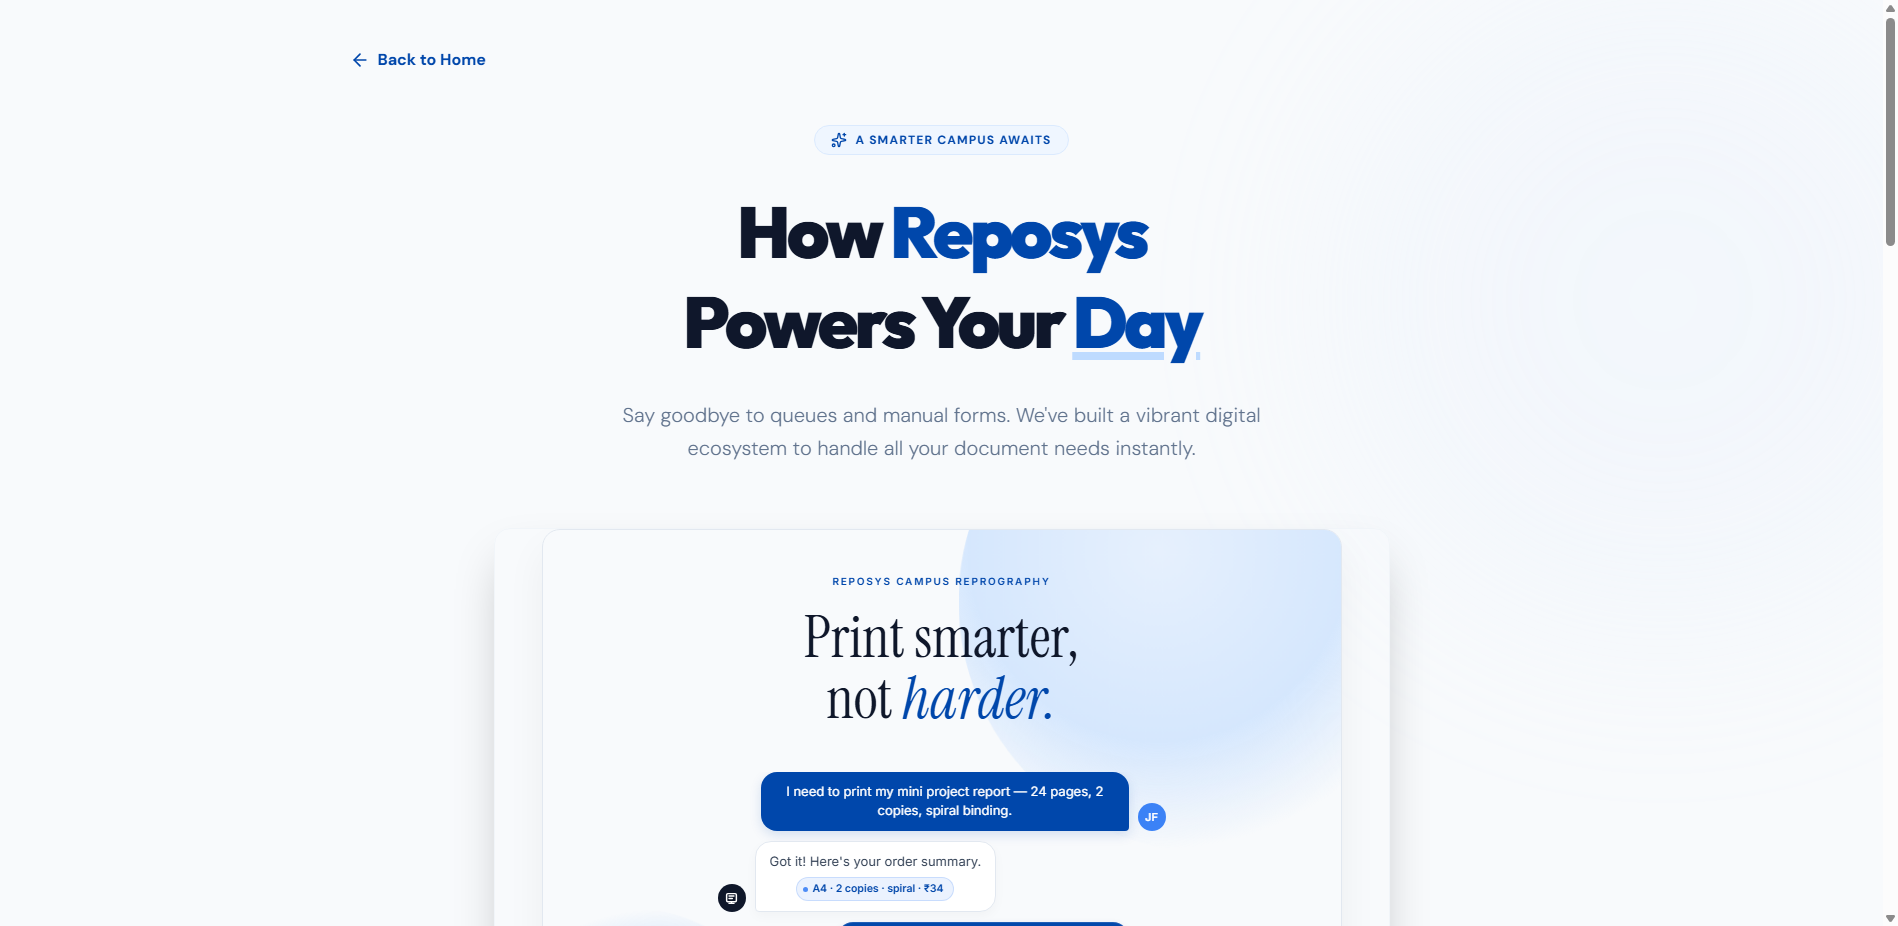
\includegraphics[width=0.85\textwidth,keepaspectratio]{figures/screen_about.png}
\caption{System Architecture Overview and About REPOSYS Portal}
\end{figure}

\newpage
\begin{figure}[H]
\centering

\includegraphics[width=0.85\textwidth,keepaspectratio]{figures/screen_contact.png}
\caption{Operational Inquiries and Customer Support Portal}
\end{figure}
\vspace{0.3in}
\begin{figure}[H]
\centering
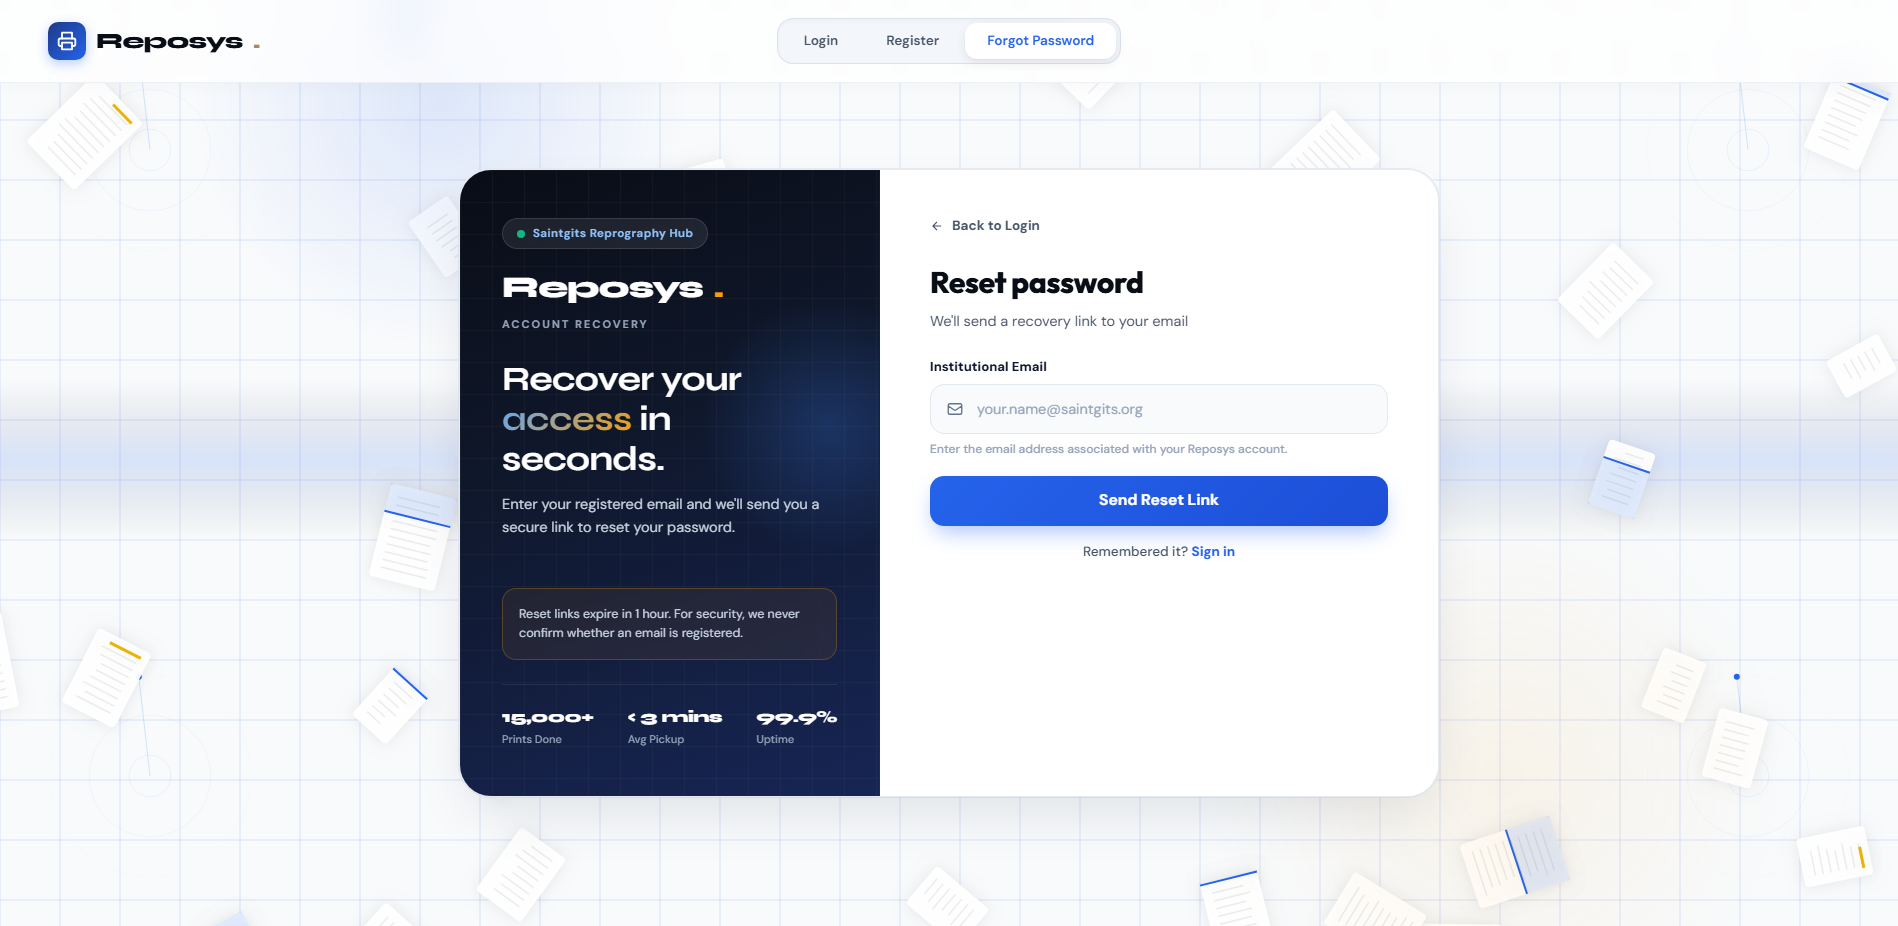
\includegraphics[width=0.85\textwidth,keepaspectratio]{figures/screen_forgot_password.png}
\caption{Account Recovery and Password Reset Workflow}
\end{figure}

\newpage
\begin{figure}[H]
\centering
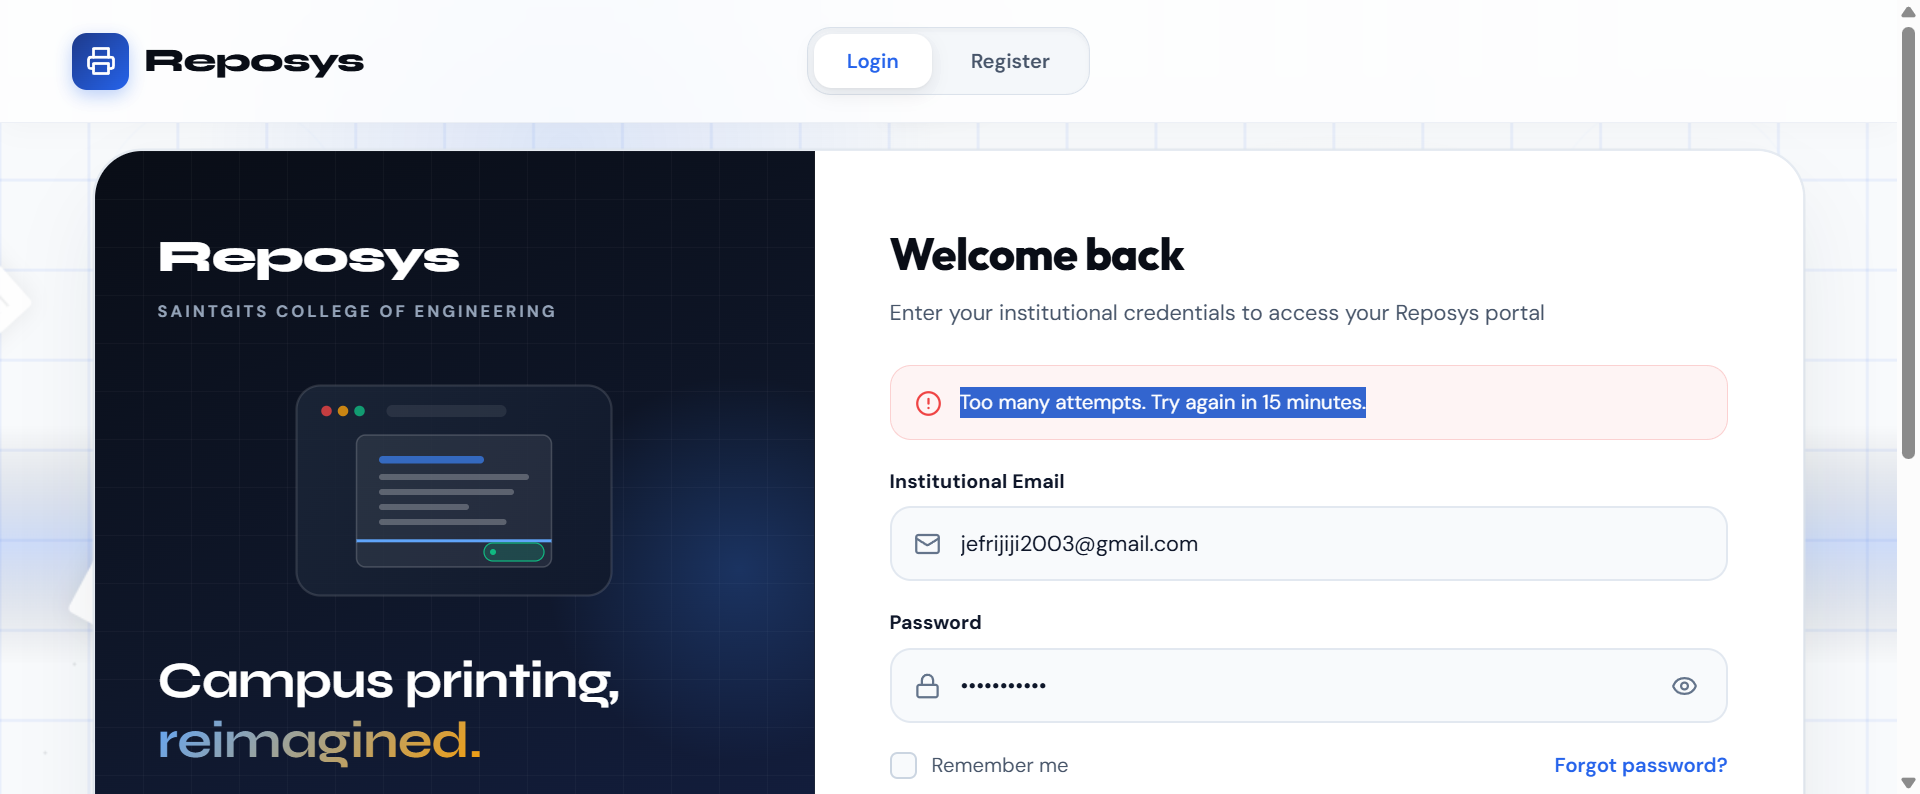
\includegraphics[width=0.85\textwidth,keepaspectratio]{figures/test_student_workflow.png}
\caption{Automated Selenium Test Run: Student Order Workflow}
\end{figure}
\vspace{0.3in}
\begin{figure}[H]
\centering
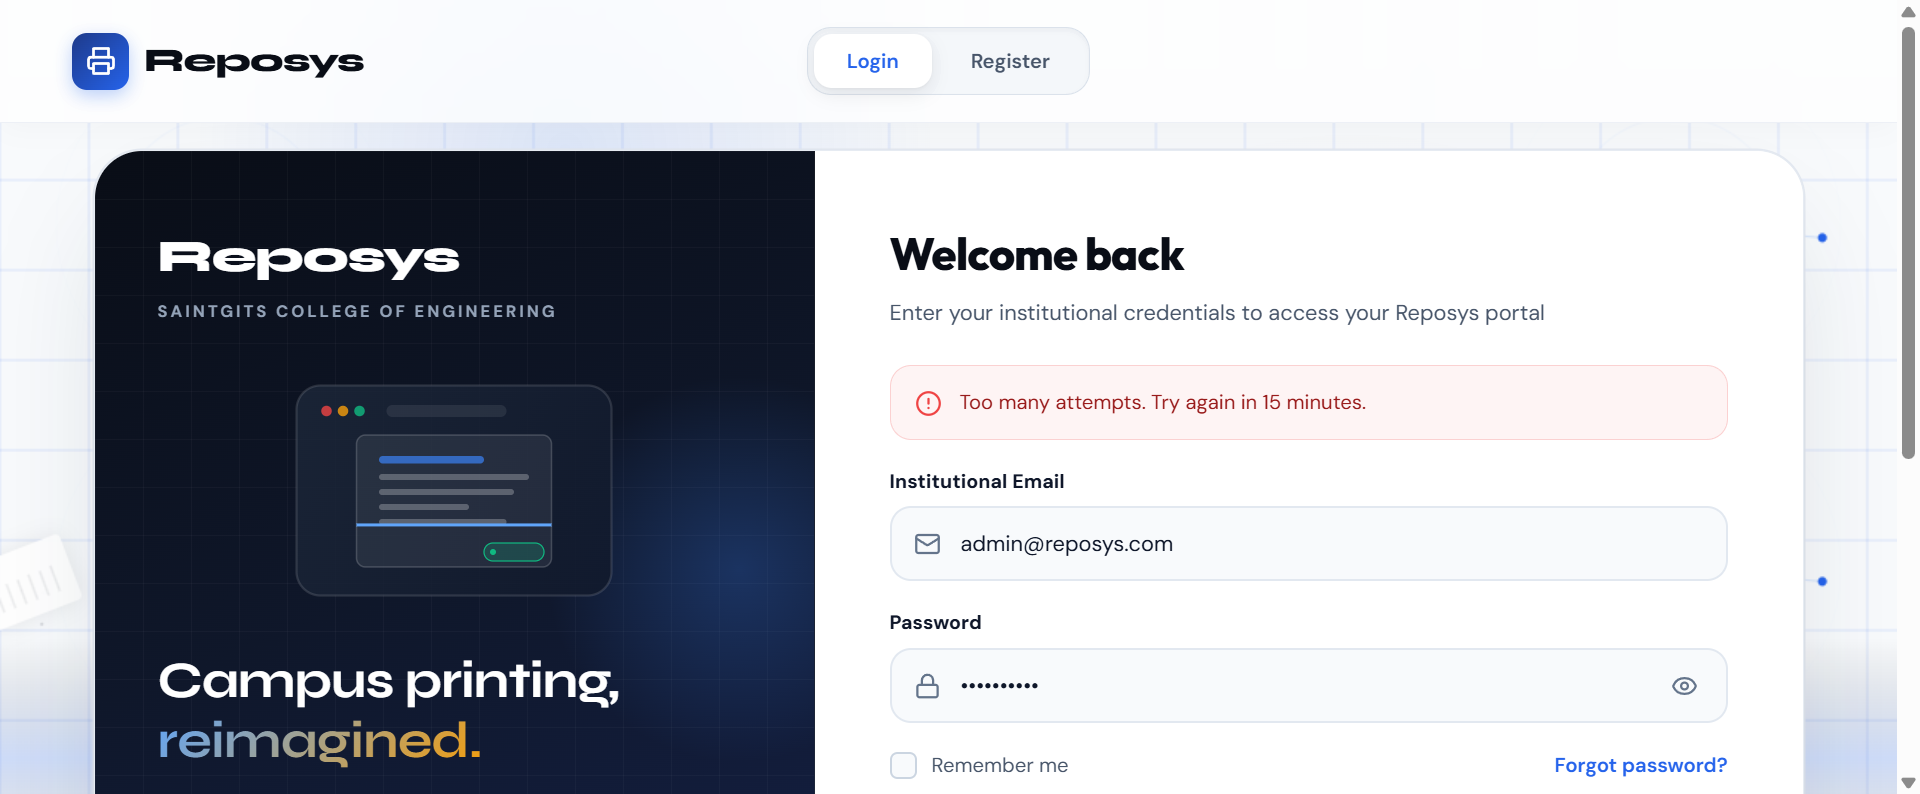
\includegraphics[width=0.85\textwidth,keepaspectratio]{figures/test_admin_access.png}
\caption{Automated Selenium Test Run: Admin Role Route Access}
\end{figure}

\newpage
\begin{figure}[H]
\centering
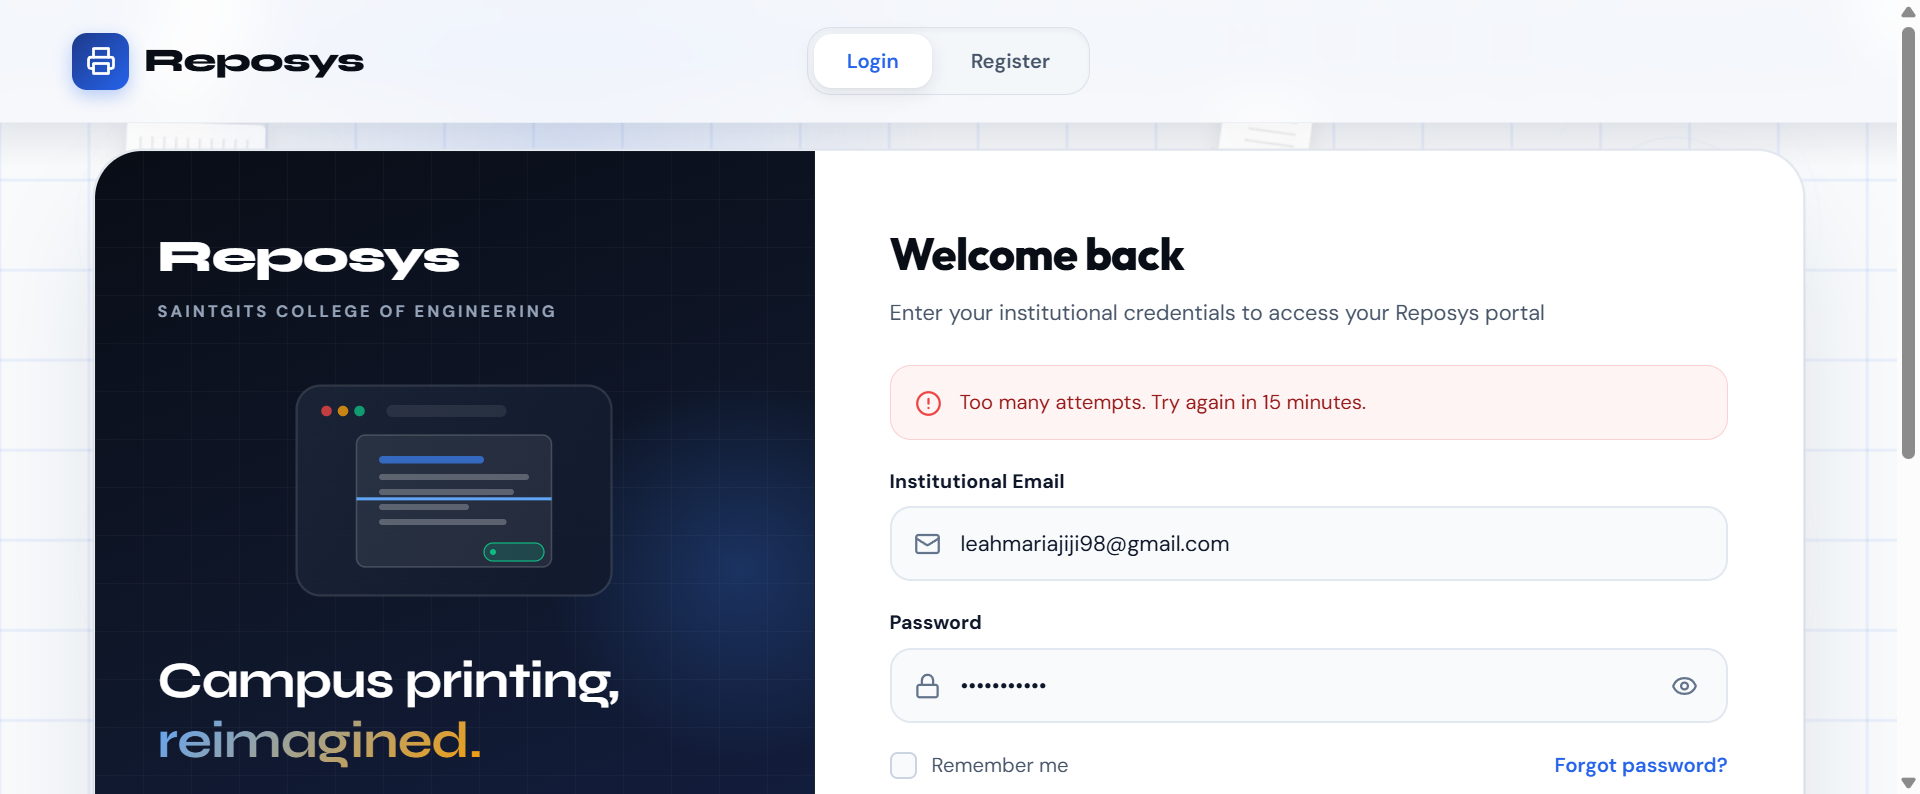
\includegraphics[width=0.85\textwidth,keepaspectratio]{figures/test_staff_access.png}
\caption{Automated Selenium Test Run: Counter Staff Queue Access}
\end{figure}
\vspace{0.3in}
\begin{figure}[H]
\centering
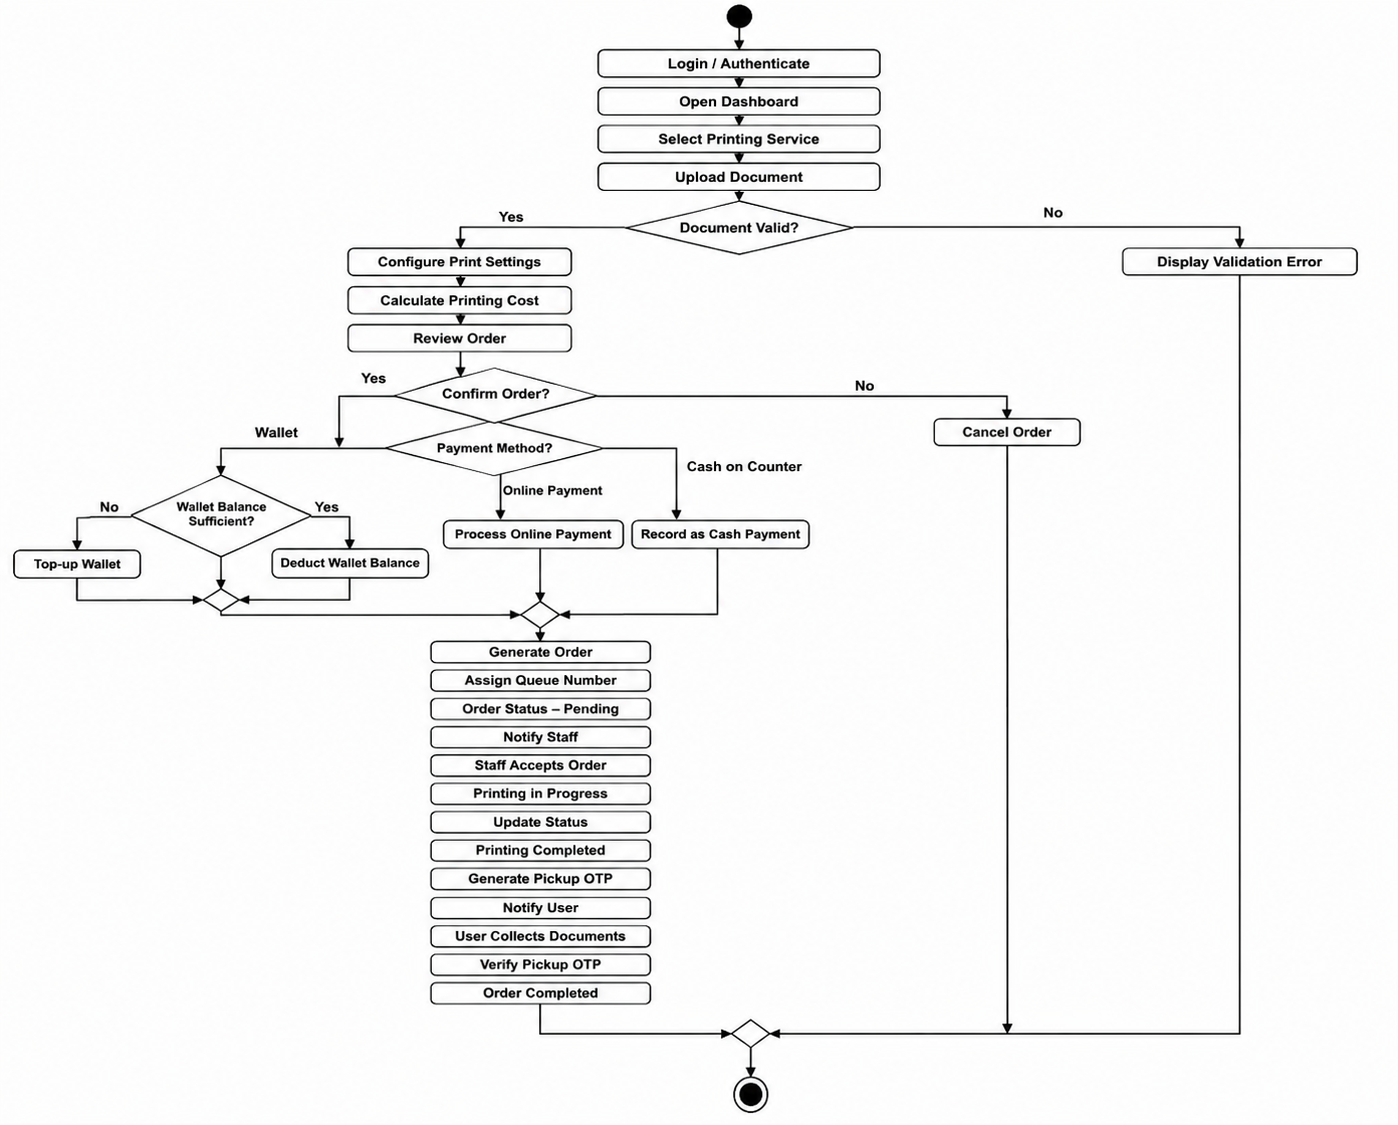
\includegraphics[width=0.85\textwidth,keepaspectratio]{figures/activity_diagram.png}
\caption{System Activity Diagram: Document Upload and Production Flow}
\end{figure}

\newpage
\begin{figure}[H]
\centering
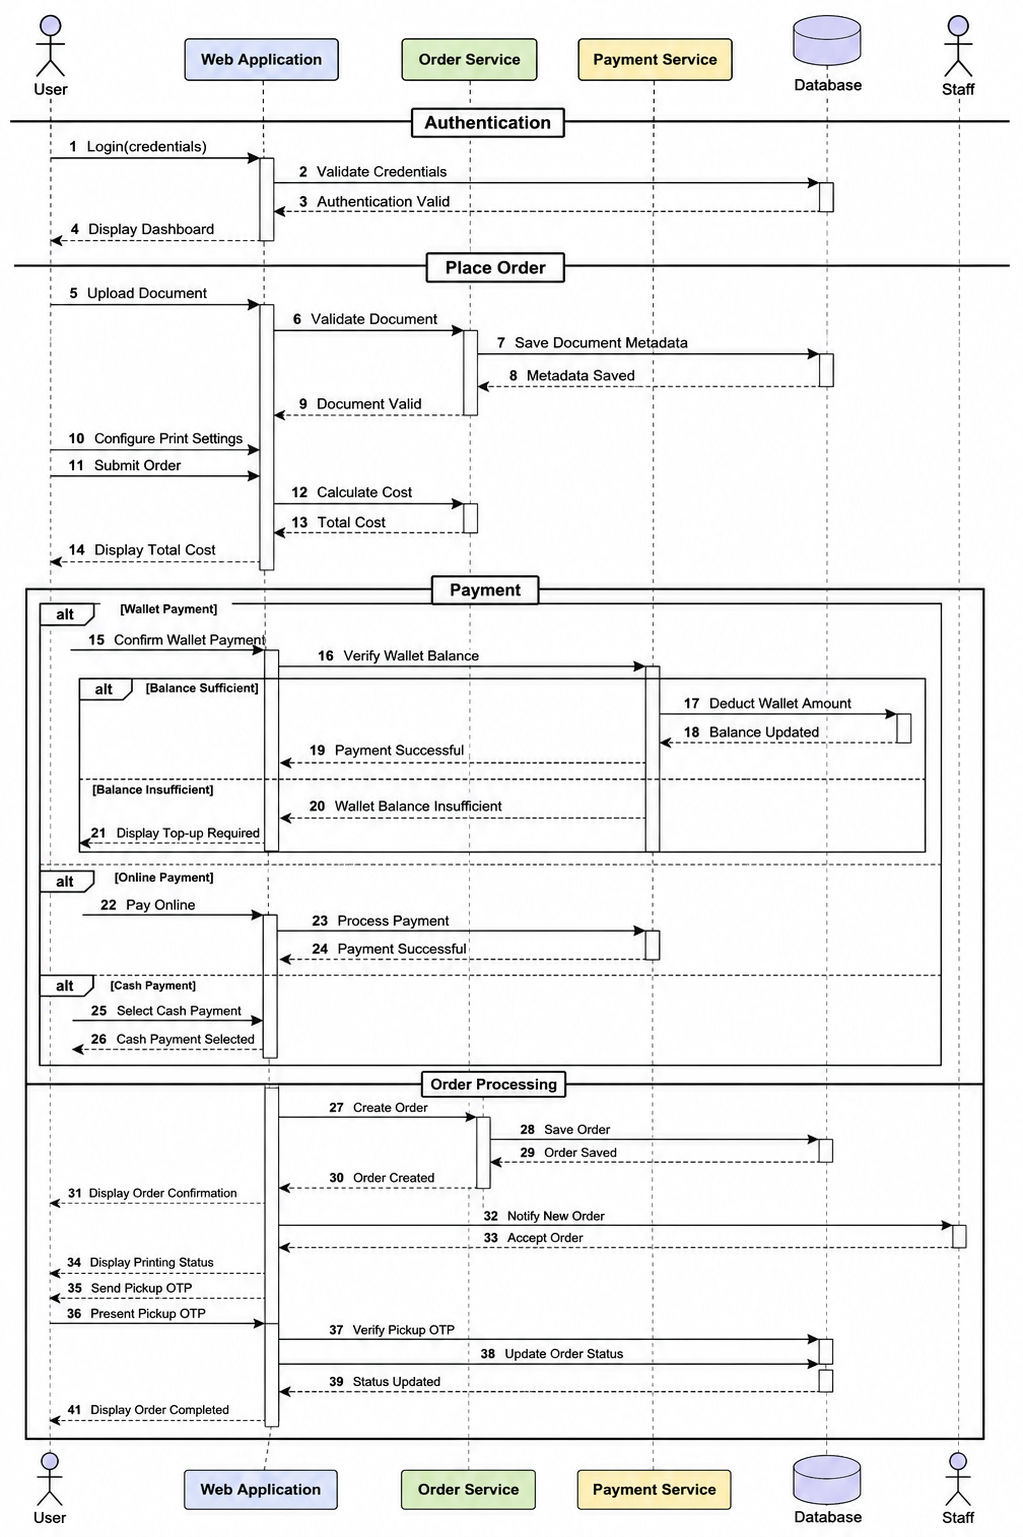
\includegraphics[width=0.85\textwidth,keepaspectratio]{figures/sequence_diagram.png}
\caption{System Sequence Diagram: Real-Time Event Dispatching}
\end{figure}

% =========================================================================
% CHAPTER 9: REFERENCES (EXACT SAMPLE PDF STRUCTURE)
% =========================================================================
\newpage
\chapter{REFERENCES}

\begin{enumerate}[leftmargin=0.35in, itemsep=8pt]
  \item APJ Abdul Kalam Technological University. (2020). \textit{Curriculum and Syllabi for Integrated Master of Computer Applications (IMCA) Programme}. KTU Academic Regulations, Thiruvananthapuram, Kerala.
  \item Cloudinary Inc. (2024). \textit{Cloudinary Node.js SDK and Media Management API Documentation}. [Online]. Available: https://cloudinary.com/documentation
  \item Electron Software Foundation. (2024). \textit{Electron Desktop Framework Documentation and Native Node.js Integration Guides}. OpenJS Foundation. [Online]. Available: https://www.electronjs.org/docs
  \item Fielding, R. T. (2000). \textit{Architectural Styles and the Design of Network-based Software Architectures} (Doctoral dissertation). University of California, Irvine.
  \item Fette, I., \& Melnikov, A. (2011). \textit{The WebSocket Protocol}. RFC 6455, Internet Engineering Task Force (IETF).
  \item Google Developers. (2024). \textit{Progressive Web Apps: High Performance Caching and Service Worker Lifecycle}. Google Web Fundamentals. [Online]. Available: https://web.dev/explore/progressive-web-apps
  \item Jones, M., Bradley, J., \& Sakimura, N. (2015). \textit{JSON Web Token (JWT)}. RFC 7519, Internet Engineering Task Force (IETF).
  \item Node.js Foundation. (2024). \textit{Node.js v20.x Long Term Support (LTS) API Specification}. OpenJS Foundation. [Online]. Available: https://nodejs.org/docs
  \item Razorpay Software Private Limited. (2024). \textit{Razorpay Payments API Specification and Webhook Signature Verification Reference}. [Online]. Available: https://razorpay.com/docs/api
  \item React Development Team. (2024). \textit{React 19 Documentation: Server Components, Hooks, and Concurrency Architecture}. Meta Open Source. [Online]. Available: https://react.dev/
  \item Saintgits College of Engineering (Autonomous). (2026). \textit{Department of Computer Applications: Mini Project Preparation Guidelines and Scrum Assessment Manual (20IMCAP501)}. Pathamuttom, Kottayam.
  \item Socket.IO Foundation. (2024). \textit{Socket.IO Client and Server Bidirectional Event Specification}. [Online]. Available: https://socket.io/docs/v4/
\end{enumerate}

\end{document}
